\documentclass{article} % For LaTeX2e
\usepackage{iclr2025,times}

% Optional math commands
%%%%% NEW MATH DEFINITIONS %%%%%

\usepackage{amsmath,amsfonts,bm}

% Mark sections of captions for referring to divisions of figures
\newcommand{\figleft}{{\em (Left)}}
\newcommand{\figcenter}{{\em (Center)}}
\newcommand{\figright}{{\em (Right)}}
\newcommand{\figtop}{{\em (Top)}}
\newcommand{\figbottom}{{\em (Bottom)}}
\newcommand{\captiona}{{\em (a)}}
\newcommand{\captionb}{{\em (b)}}
\newcommand{\captionc}{{\em (c)}}
\newcommand{\captiond}{{\em (d)}}

% Highlight a newly defined term
\newcommand{\newterm}[1]{{\bf #1}}


% Figure reference, lower-case.
\def\figref#1{figure~\ref{#1}}
% Figure reference, capital. For start of sentence
\def\Figref#1{Figure~\ref{#1}}
\def\twofigref#1#2{figures \ref{#1} and \ref{#2}}
\def\quadfigref#1#2#3#4{figures \ref{#1}, \ref{#2}, \ref{#3} and \ref{#4}}
% Section reference, lower-case.
\def\secref#1{section~\ref{#1}}
% Section reference, capital.
\def\Secref#1{Section~\ref{#1}}
% Reference to two sections.
\def\twosecrefs#1#2{sections \ref{#1} and \ref{#2}}
% Reference to three sections.
\def\secrefs#1#2#3{sections \ref{#1}, \ref{#2} and \ref{#3}}
% Reference to an equation, lower-case.
\def\eqref#1{equation~\ref{#1}}
% Reference to an equation, upper case
\def\Eqref#1{Equation~\ref{#1}}
% A raw reference to an equation---avoid using if possible
\def\plaineqref#1{\ref{#1}}
% Reference to a chapter, lower-case.
\def\chapref#1{chapter~\ref{#1}}
% Reference to an equation, upper case.
\def\Chapref#1{Chapter~\ref{#1}}
% Reference to a range of chapters
\def\rangechapref#1#2{chapters\ref{#1}--\ref{#2}}
% Reference to an algorithm, lower-case.
\def\algref#1{algorithm~\ref{#1}}
% Reference to an algorithm, upper case.
\def\Algref#1{Algorithm~\ref{#1}}
\def\twoalgref#1#2{algorithms \ref{#1} and \ref{#2}}
\def\Twoalgref#1#2{Algorithms \ref{#1} and \ref{#2}}
% Reference to a part, lower case
\def\partref#1{part~\ref{#1}}
% Reference to a part, upper case
\def\Partref#1{Part~\ref{#1}}
\def\twopartref#1#2{parts \ref{#1} and \ref{#2}}

\def\ceil#1{\lceil #1 \rceil}
\def\floor#1{\lfloor #1 \rfloor}
\def\1{\bm{1}}
\newcommand{\train}{\mathcal{D}}
\newcommand{\valid}{\mathcal{D_{\mathrm{valid}}}}
\newcommand{\test}{\mathcal{D_{\mathrm{test}}}}

\def\eps{{\epsilon}}


% Random variables
\def\reta{{\textnormal{$\eta$}}}
\def\ra{{\textnormal{a}}}
\def\rb{{\textnormal{b}}}
\def\rc{{\textnormal{c}}}
\def\rd{{\textnormal{d}}}
\def\re{{\textnormal{e}}}
\def\rf{{\textnormal{f}}}
\def\rg{{\textnormal{g}}}
\def\rh{{\textnormal{h}}}
\def\ri{{\textnormal{i}}}
\def\rj{{\textnormal{j}}}
\def\rk{{\textnormal{k}}}
\def\rl{{\textnormal{l}}}
% rm is already a command, just don't name any random variables m
\def\rn{{\textnormal{n}}}
\def\ro{{\textnormal{o}}}
\def\rp{{\textnormal{p}}}
\def\rq{{\textnormal{q}}}
\def\rr{{\textnormal{r}}}
\def\rs{{\textnormal{s}}}
\def\rt{{\textnormal{t}}}
\def\ru{{\textnormal{u}}}
\def\rv{{\textnormal{v}}}
\def\rw{{\textnormal{w}}}
\def\rx{{\textnormal{x}}}
\def\ry{{\textnormal{y}}}
\def\rz{{\textnormal{z}}}

% Random vectors
\def\rvepsilon{{\mathbf{\epsilon}}}
\def\rvtheta{{\mathbf{\theta}}}
\def\rva{{\mathbf{a}}}
\def\rvb{{\mathbf{b}}}
\def\rvc{{\mathbf{c}}}
\def\rvd{{\mathbf{d}}}
\def\rve{{\mathbf{e}}}
\def\rvf{{\mathbf{f}}}
\def\rvg{{\mathbf{g}}}
\def\rvh{{\mathbf{h}}}
\def\rvu{{\mathbf{i}}}
\def\rvj{{\mathbf{j}}}
\def\rvk{{\mathbf{k}}}
\def\rvl{{\mathbf{l}}}
\def\rvm{{\mathbf{m}}}
\def\rvn{{\mathbf{n}}}
\def\rvo{{\mathbf{o}}}
\def\rvp{{\mathbf{p}}}
\def\rvq{{\mathbf{q}}}
\def\rvr{{\mathbf{r}}}
\def\rvs{{\mathbf{s}}}
\def\rvt{{\mathbf{t}}}
\def\rvu{{\mathbf{u}}}
\def\rvv{{\mathbf{v}}}
\def\rvw{{\mathbf{w}}}
\def\rvx{{\mathbf{x}}}
\def\rvy{{\mathbf{y}}}
\def\rvz{{\mathbf{z}}}

% Elements of random vectors
\def\erva{{\textnormal{a}}}
\def\ervb{{\textnormal{b}}}
\def\ervc{{\textnormal{c}}}
\def\ervd{{\textnormal{d}}}
\def\erve{{\textnormal{e}}}
\def\ervf{{\textnormal{f}}}
\def\ervg{{\textnormal{g}}}
\def\ervh{{\textnormal{h}}}
\def\ervi{{\textnormal{i}}}
\def\ervj{{\textnormal{j}}}
\def\ervk{{\textnormal{k}}}
\def\ervl{{\textnormal{l}}}
\def\ervm{{\textnormal{m}}}
\def\ervn{{\textnormal{n}}}
\def\ervo{{\textnormal{o}}}
\def\ervp{{\textnormal{p}}}
\def\ervq{{\textnormal{q}}}
\def\ervr{{\textnormal{r}}}
\def\ervs{{\textnormal{s}}}
\def\ervt{{\textnormal{t}}}
\def\ervu{{\textnormal{u}}}
\def\ervv{{\textnormal{v}}}
\def\ervw{{\textnormal{w}}}
\def\ervx{{\textnormal{x}}}
\def\ervy{{\textnormal{y}}}
\def\ervz{{\textnormal{z}}}

% Random matrices
\def\rmA{{\mathbf{A}}}
\def\rmB{{\mathbf{B}}}
\def\rmC{{\mathbf{C}}}
\def\rmD{{\mathbf{D}}}
\def\rmE{{\mathbf{E}}}
\def\rmF{{\mathbf{F}}}
\def\rmG{{\mathbf{G}}}
\def\rmH{{\mathbf{H}}}
\def\rmI{{\mathbf{I}}}
\def\rmJ{{\mathbf{J}}}
\def\rmK{{\mathbf{K}}}
\def\rmL{{\mathbf{L}}}
\def\rmM{{\mathbf{M}}}
\def\rmN{{\mathbf{N}}}
\def\rmO{{\mathbf{O}}}
\def\rmP{{\mathbf{P}}}
\def\rmQ{{\mathbf{Q}}}
\def\rmR{{\mathbf{R}}}
\def\rmS{{\mathbf{S}}}
\def\rmT{{\mathbf{T}}}
\def\rmU{{\mathbf{U}}}
\def\rmV{{\mathbf{V}}}
\def\rmW{{\mathbf{W}}}
\def\rmX{{\mathbf{X}}}
\def\rmY{{\mathbf{Y}}}
\def\rmZ{{\mathbf{Z}}}

% Elements of random matrices
\def\ermA{{\textnormal{A}}}
\def\ermB{{\textnormal{B}}}
\def\ermC{{\textnormal{C}}}
\def\ermD{{\textnormal{D}}}
\def\ermE{{\textnormal{E}}}
\def\ermF{{\textnormal{F}}}
\def\ermG{{\textnormal{G}}}
\def\ermH{{\textnormal{H}}}
\def\ermI{{\textnormal{I}}}
\def\ermJ{{\textnormal{J}}}
\def\ermK{{\textnormal{K}}}
\def\ermL{{\textnormal{L}}}
\def\ermM{{\textnormal{M}}}
\def\ermN{{\textnormal{N}}}
\def\ermO{{\textnormal{O}}}
\def\ermP{{\textnormal{P}}}
\def\ermQ{{\textnormal{Q}}}
\def\ermR{{\textnormal{R}}}
\def\ermS{{\textnormal{S}}}
\def\ermT{{\textnormal{T}}}
\def\ermU{{\textnormal{U}}}
\def\ermV{{\textnormal{V}}}
\def\ermW{{\textnormal{W}}}
\def\ermX{{\textnormal{X}}}
\def\ermY{{\textnormal{Y}}}
\def\ermZ{{\textnormal{Z}}}

% Vectors
\def\vzero{{\bm{0}}}
\def\vone{{\bm{1}}}
\def\vmu{{\bm{\mu}}}
\def\vtheta{{\bm{\theta}}}
\def\va{{\bm{a}}}
\def\vb{{\bm{b}}}
\def\vc{{\bm{c}}}
\def\vd{{\bm{d}}}
\def\ve{{\bm{e}}}
\def\vf{{\bm{f}}}
\def\vg{{\bm{g}}}
\def\vh{{\bm{h}}}
\def\vi{{\bm{i}}}
\def\vj{{\bm{j}}}
\def\vk{{\bm{k}}}
\def\vl{{\bm{l}}}
\def\vm{{\bm{m}}}
\def\vn{{\bm{n}}}
\def\vo{{\bm{o}}}
\def\vp{{\bm{p}}}
\def\vq{{\bm{q}}}
\def\vr{{\bm{r}}}
\def\vs{{\bm{s}}}
\def\vt{{\bm{t}}}
\def\vu{{\bm{u}}}
\def\vv{{\bm{v}}}
\def\vw{{\bm{w}}}
\def\vx{{\bm{x}}}
\def\vy{{\bm{y}}}
\def\vz{{\bm{z}}}

% Elements of vectors
\def\evalpha{{\alpha}}
\def\evbeta{{\beta}}
\def\evepsilon{{\epsilon}}
\def\evlambda{{\lambda}}
\def\evomega{{\omega}}
\def\evmu{{\mu}}
\def\evpsi{{\psi}}
\def\evsigma{{\sigma}}
\def\evtheta{{\theta}}
\def\eva{{a}}
\def\evb{{b}}
\def\evc{{c}}
\def\evd{{d}}
\def\eve{{e}}
\def\evf{{f}}
\def\evg{{g}}
\def\evh{{h}}
\def\evi{{i}}
\def\evj{{j}}
\def\evk{{k}}
\def\evl{{l}}
\def\evm{{m}}
\def\evn{{n}}
\def\evo{{o}}
\def\evp{{p}}
\def\evq{{q}}
\def\evr{{r}}
\def\evs{{s}}
\def\evt{{t}}
\def\evu{{u}}
\def\evv{{v}}
\def\evw{{w}}
\def\evx{{x}}
\def\evy{{y}}
\def\evz{{z}}

% Matrix
\def\mA{{\bm{A}}}
\def\mB{{\bm{B}}}
\def\mC{{\bm{C}}}
\def\mD{{\bm{D}}}
\def\mE{{\bm{E}}}
\def\mF{{\bm{F}}}
\def\mG{{\bm{G}}}
\def\mH{{\bm{H}}}
\def\mI{{\bm{I}}}
\def\mJ{{\bm{J}}}
\def\mK{{\bm{K}}}
\def\mL{{\bm{L}}}
\def\mM{{\bm{M}}}
\def\mN{{\bm{N}}}
\def\mO{{\bm{O}}}
\def\mP{{\bm{P}}}
\def\mQ{{\bm{Q}}}
\def\mR{{\bm{R}}}
\def\mS{{\bm{S}}}
\def\mT{{\bm{T}}}
\def\mU{{\bm{U}}}
\def\mV{{\bm{V}}}
\def\mW{{\bm{W}}}
\def\mX{{\bm{X}}}
\def\mY{{\bm{Y}}}
\def\mZ{{\bm{Z}}}
\def\mBeta{{\bm{\beta}}}
\def\mPhi{{\bm{\Phi}}}
\def\mLambda{{\bm{\Lambda}}}
\def\mSigma{{\bm{\Sigma}}}

% Tensor
\DeclareMathAlphabet{\mathsfit}{\encodingdefault}{\sfdefault}{m}{sl}
\SetMathAlphabet{\mathsfit}{bold}{\encodingdefault}{\sfdefault}{bx}{n}
\newcommand{\tens}[1]{\bm{\mathsfit{#1}}}
\def\tA{{\tens{A}}}
\def\tB{{\tens{B}}}
\def\tC{{\tens{C}}}
\def\tD{{\tens{D}}}
\def\tE{{\tens{E}}}
\def\tF{{\tens{F}}}
\def\tG{{\tens{G}}}
\def\tH{{\tens{H}}}
\def\tI{{\tens{I}}}
\def\tJ{{\tens{J}}}
\def\tK{{\tens{K}}}
\def\tL{{\tens{L}}}
\def\tM{{\tens{M}}}
\def\tN{{\tens{N}}}
\def\tO{{\tens{O}}}
\def\tP{{\tens{P}}}
\def\tQ{{\tens{Q}}}
\def\tR{{\tens{R}}}
\def\tS{{\tens{S}}}
\def\tT{{\tens{T}}}
\def\tU{{\tens{U}}}
\def\tV{{\tens{V}}}
\def\tW{{\tens{W}}}
\def\tX{{\tens{X}}}
\def\tY{{\tens{Y}}}
\def\tZ{{\tens{Z}}}


% Graph
\def\gA{{\mathcal{A}}}
\def\gB{{\mathcal{B}}}
\def\gC{{\mathcal{C}}}
\def\gD{{\mathcal{D}}}
\def\gE{{\mathcal{E}}}
\def\gF{{\mathcal{F}}}
\def\gG{{\mathcal{G}}}
\def\gH{{\mathcal{H}}}
\def\gI{{\mathcal{I}}}
\def\gJ{{\mathcal{J}}}
\def\gK{{\mathcal{K}}}
\def\gL{{\mathcal{L}}}
\def\gM{{\mathcal{M}}}
\def\gN{{\mathcal{N}}}
\def\gO{{\mathcal{O}}}
\def\gP{{\mathcal{P}}}
\def\gQ{{\mathcal{Q}}}
\def\gR{{\mathcal{R}}}
\def\gS{{\mathcal{S}}}
\def\gT{{\mathcal{T}}}
\def\gU{{\mathcal{U}}}
\def\gV{{\mathcal{V}}}
\def\gW{{\mathcal{W}}}
\def\gX{{\mathcal{X}}}
\def\gY{{\mathcal{Y}}}
\def\gZ{{\mathcal{Z}}}

% Sets
\def\sA{{\mathbb{A}}}
\def\sB{{\mathbb{B}}}
\def\sC{{\mathbb{C}}}
\def\sD{{\mathbb{D}}}
% Don't use a set called E, because this would be the same as our symbol
% for expectation.
\def\sF{{\mathbb{F}}}
\def\sG{{\mathbb{G}}}
\def\sH{{\mathbb{H}}}
\def\sI{{\mathbb{I}}}
\def\sJ{{\mathbb{J}}}
\def\sK{{\mathbb{K}}}
\def\sL{{\mathbb{L}}}
\def\sM{{\mathbb{M}}}
\def\sN{{\mathbb{N}}}
\def\sO{{\mathbb{O}}}
\def\sP{{\mathbb{P}}}
\def\sQ{{\mathbb{Q}}}
\def\sR{{\mathbb{R}}}
\def\sS{{\mathbb{S}}}
\def\sT{{\mathbb{T}}}
\def\sU{{\mathbb{U}}}
\def\sV{{\mathbb{V}}}
\def\sW{{\mathbb{W}}}
\def\sX{{\mathbb{X}}}
\def\sY{{\mathbb{Y}}}
\def\sZ{{\mathbb{Z}}}

% Entries of a matrix
\def\emLambda{{\Lambda}}
\def\emA{{A}}
\def\emB{{B}}
\def\emC{{C}}
\def\emD{{D}}
\def\emE{{E}}
\def\emF{{F}}
\def\emG{{G}}
\def\emH{{H}}
\def\emI{{I}}
\def\emJ{{J}}
\def\emK{{K}}
\def\emL{{L}}
\def\emM{{M}}
\def\emN{{N}}
\def\emO{{O}}
\def\emP{{P}}
\def\emQ{{Q}}
\def\emR{{R}}
\def\emS{{S}}
\def\emT{{T}}
\def\emU{{U}}
\def\emV{{V}}
\def\emW{{W}}
\def\emX{{X}}
\def\emY{{Y}}
\def\emZ{{Z}}
\def\emSigma{{\Sigma}}

% entries of a tensor
% Same font as tensor, without \bm wrapper
\newcommand{\etens}[1]{\mathsfit{#1}}
\def\etLambda{{\etens{\Lambda}}}
\def\etA{{\etens{A}}}
\def\etB{{\etens{B}}}
\def\etC{{\etens{C}}}
\def\etD{{\etens{D}}}
\def\etE{{\etens{E}}}
\def\etF{{\etens{F}}}
\def\etG{{\etens{G}}}
\def\etH{{\etens{H}}}
\def\etI{{\etens{I}}}
\def\etJ{{\etens{J}}}
\def\etK{{\etens{K}}}
\def\etL{{\etens{L}}}
\def\etM{{\etens{M}}}
\def\etN{{\etens{N}}}
\def\etO{{\etens{O}}}
\def\etP{{\etens{P}}}
\def\etQ{{\etens{Q}}}
\def\etR{{\etens{R}}}
\def\etS{{\etens{S}}}
\def\etT{{\etens{T}}}
\def\etU{{\etens{U}}}
\def\etV{{\etens{V}}}
\def\etW{{\etens{W}}}
\def\etX{{\etens{X}}}
\def\etY{{\etens{Y}}}
\def\etZ{{\etens{Z}}}

% The true underlying data generating distribution
\newcommand{\pdata}{p_{\rm{data}}}
% The empirical distribution defined by the training set
\newcommand{\ptrain}{\hat{p}_{\rm{data}}}
\newcommand{\Ptrain}{\hat{P}_{\rm{data}}}
% The model distribution
\newcommand{\pmodel}{p_{\rm{model}}}
\newcommand{\Pmodel}{P_{\rm{model}}}
\newcommand{\ptildemodel}{\tilde{p}_{\rm{model}}}
% Stochastic autoencoder distributions
\newcommand{\pencode}{p_{\rm{encoder}}}
\newcommand{\pdecode}{p_{\rm{decoder}}}
\newcommand{\precons}{p_{\rm{reconstruct}}}

\newcommand{\laplace}{\mathrm{Laplace}} % Laplace distribution

\newcommand{\E}{\mathbb{E}}
\newcommand{\Ls}{\mathcal{L}}
\newcommand{\R}{\mathbb{R}}
\newcommand{\emp}{\tilde{p}}
\newcommand{\lr}{\alpha}
\newcommand{\reg}{\lambda}
\newcommand{\rect}{\mathrm{rectifier}}
\newcommand{\softmax}{\mathrm{softmax}}
\newcommand{\sigmoid}{\sigma}
\newcommand{\softplus}{\zeta}
\newcommand{\KL}{D_{\mathrm{KL}}}
\newcommand{\Var}{\mathrm{Var}}
\newcommand{\standarderror}{\mathrm{SE}}
\newcommand{\Cov}{\mathrm{Cov}}
% Wolfram Mathworld says $L^2$ is for function spaces and $\ell^2$ is for vectors
% But then they seem to use $L^2$ for vectors throughout the site, and so does
% wikipedia.
\newcommand{\normlzero}{L^0}
\newcommand{\normlone}{L^1}
\newcommand{\normltwo}{L^2}
\newcommand{\normlp}{L^p}
\newcommand{\normmax}{L^\infty}

\newcommand{\parents}{Pa} % See usage in notation.tex. Chosen to match Daphne's book.

\DeclareMathOperator*{\argmax}{arg\,max}
\DeclareMathOperator*{\argmin}{arg\,min}

\DeclareMathOperator{\sign}{sign}
\DeclareMathOperator{\Tr}{Tr}
\let\ab\allowbreak


\usepackage{hyperref}
\usepackage{url}
\usepackage{graphicx}
\usepackage{subfigure}
\usepackage{booktabs}
\usepackage{amsmath,amssymb,mathtools}
\usepackage[capitalize,noabbrev]{cleveref}

\graphicspath{{../figures/}} % To reference your generated figures

\begin{filecontents}{references.bib}
@book{goodfellow2016deep,
  title={Deep learning},
  author={Goodfellow, Ian and Bengio, Yoshua and Courville, Aaron},
  volume={1},
  year={2016},
  publisher={MIT Press}
}
@article{wang2018glueam,
  author = {Alex Wang and Amanpreet Singh and Julian Michael and Felix Hill and Omer Levy and Samuel R. Bowman},
  booktitle = {BlackboxNLP@EMNLP},
  pages = {353--355},
  title = {{GLUE}: A Multi-Task Benchmark and Analysis Platform for Natural Language Understanding},
  year = {2018}
}
@article{gupta2024twinadaptcl,
  author = {Ragini Gupta and Beitong Tian and Yaohui Wang and Klara Nahrstedt},
  booktitle = {Future Internet},
  journal = {Future Internet},
  pages = {239},
  title = {TWIN-ADAPT: Continuous Learning for Digital Twin-Enabled Online Anomaly Classification in IoT-Driven Smart Labs},
  volume = {16},
  year = {2024}
}
@article{recht2019doic,
  author = {B. Recht and R. Roelofs and Ludwig Schmidt and Vaishaal Shankar},
  booktitle = {International Conference on Machine Learning},
  pages = {5389--5400},
  title = {Do ImageNet Classifiers Generalize to ImageNet?},
  year = {2019}
}
@article{rajpurkar2016squad1q,
  author = {Pranav Rajpurkar and Jian Zhang and Konstantin Lopyrev and Percy Liang},
  booktitle = {Conference on Empirical Methods in Natural Language Processing},
  pages = {2383--2392},
  title = {{SQuAD}: 100{,}000+ Questions for Machine Comprehension of Text},
  year = {2016}
}
@article{karras2019analyzingai,
  author = {Tero Karras and S. Laine and M. Aittala and Janne Hellsten and J. Lehtinen and Timo Aila},
  booktitle = {IEEE/CVF Conference on Computer Vision and Pattern Recognition},
  pages = {8107--8116},
  title = {Analyzing and Improving the Image Quality of StyleGAN},
  year = {2019}
}
@article{heusel2017ganstb,
  author = {M. Heusel and Hubert Ramsauer and Thomas Unterthiner and Bernhard Nessler and Sepp Hochreiter},
  booktitle = {Neural Information Processing Systems},
  pages = {6626--6637},
  title = {GANs Trained by a Two Time-Scale Update Rule Converge to a Local Nash Equilibrium},
  year = {2017}
}
@article{radford2019languagema,
  author = {Alec Radford and Jeff Wu and R. Child and D. Luan and Dario Amodei and I. Sutskever},
  title = {Language Models are Unsupervised Multitask Learners},
  year = {2019}
}
@article{lakshminarayanan2016simpleas,
  author = {Balaji Lakshminarayanan and A. Pritzel and C. Blundell},
  booktitle = {Neural Information Processing Systems},
  pages = {6402--6413},
  title = {Simple and Scalable Predictive Uncertainty Estimation using Deep Ensembles},
  year = {2016}
}
@article{gretton2012akt,
  author = {A. Gretton and Karsten M. Borgwardt and M. Rasch and B. Schölkopf and Alex Smola},
  booktitle = {Journal of Machine Learning Research},
  pages = {723--773},
  title = {A Kernel Two-Sample Test},
  volume = {13},
  year = {2012}
}
@article{wang2019superglueas,
  author = {Alex Wang and Yada Pruksachatkun and Nikita Nangia and Amanpreet Singh and Julian Michael and Felix Hill and Omer Levy and Samuel R. Bowman},
  booktitle = {Neural Information Processing Systems},
  title = {SuperGLUE: A Stickier Benchmark for General-Purpose Language Understanding Systems},
  year = {2019}
}
@inproceedings{lecun1998gradientbasedla,
  author = {Yann LeCun and L. Bottou and Yoshua Bengio and P. Haffner},
  booktitle = {Proceedings of the IEEE},
  pages = {2278--2324},
  title = {Gradient-based learning applied to document recognition},
  volume = {86},
  year = {1998}
}
@inproceedings{krizhevsky2009learningml,
  author = {A. Krizhevsky},
  title = {Learning Multiple Layers of Features from Tiny Images},
  year = {2009}
}
@article{deng2009imagenetal,
  author = {Jia Deng and Wei Dong and R. Socher and Li-Jia Li and Li Fei-Fei},
  booktitle = {2009 IEEE Conference on Computer Vision and Pattern Recognition},
  pages = {248--255},
  title = {ImageNet: A large-scale hierarchical image database},
  year = {2009}
}
@article{goodfellow2014explainingah,
  author = {I. Goodfellow and Jonathon Shlens and Christian Szegedy},
  booktitle = {International Conference on Learning Representations},
  title = {Explaining and Harnessing Adversarial Examples},
  volume = {abs/1412.6572},
  year = {2014}
}
\end{filecontents}

\title{The Lifecycle of ML Benchmarks: Quantifying and Counteracting Dataset Aging}

\author{Anonymous}

\begin{document}
\maketitle

\begin{abstract}
Machine learning benchmarks like MNIST, CIFAR-10, ImageNet, GLUE, and SQuAD have driven rapid model improvements, but as architectures advance and real-world distributions drift, static benchmarks lose discriminative power and relevance. We introduce \emph{benchmark decay}, a measurable decline in a dataset's ability to distinguish competitive models over time. We propose three decay metrics—performance saturation gap, year-over-year challenge drop, and a distributional shift index—and apply them retrospectively to canonical vision and language benchmarks using leaderboard archives and embeddings. We then design a lightweight synthetic \emph{rejuvenation pipeline} that targets high-uncertainty regions via conditional generative models, filters samples by FID/perplexity, and injects $<5\%$ new test examples. In two case studies (MNIST and text classification), we quantify decay trends, show mid-training epochs maximize model discrimination, and demonstrate that automated synthetic additions partially restore challenge without manual reannotation. Our findings highlight pervasive benchmark aging and chart a path toward dynamic, sustainable evaluation.
\end{abstract}

\section{Introduction}
Static benchmarks underpin progress in deep learning, but they are not immune to \emph{aging}: as new models saturate performance and real data shifts, benchmarks become trivial or less representative of current tasks. Empirical shifts in CIFAR-10 and ImageNet have been documented \citep{recht2019doic}, and GLUE saturation prompted SuperGLUE \citep{wang2019superglueas}. Yet practitioners lack a unified framework to quantify decay or refresh benchmarks cost-effectively, risking overstated progress and models unprepared for evolving real-world data.

We address this by introducing \emph{benchmark decay metrics} and a \emph{synthetic rejuvenation pipeline}. Our contributions are: (1) a quantitative toolkit to measure saturation gaps, year-over-year drops, and distributional shifts on static datasets; (2) a GAN/GPT-based pipeline that generates and filters challenging test samples, adding $<5\%$ synthetic data to restore discrimination; (3) case studies on MNIST rotation robustness and three text tasks (AG News, SST2, Yelp Polarity) that reveal decaying discrimination and demonstrate preliminary synthetic rejuvenation effects.

\section{Related Work}
Domain and concept drift in streaming data has been extensively studied \citep{gupta2024twinadaptcl}, but static benchmarks receive less maintenance. Benchmark re-splits for CIFAR-10 and ImageNet highlight generalization gaps \citep{recht2019doic}. In NLP, GLUE \citep{wang2018glueam} saturation led to SuperGLUE \citep{wang2019superglueas}. Adversarial and synthetic example generation \citep{goodfellow2014explainingah, heusel2017ganstb} and deep ensembles for uncertainty estimation \citep{lakshminarayanan2016simpleas} each tackle parts of the challenge. We unify these strands to quantify static benchmark decay and propose an automated refresh workflow.

\section{Method}
Given a static benchmark $\mathcal{D}=(\mathcal{X},\mathcal{Y})$ with historical model scores, we define:
\emph{Saturation gap} as the difference between a human ceiling and the top model accuracy over time; \emph{challenge drop} as the annual change in top-$k$ accuracy; and \emph{distribution shift} as the MMD statistic between original and current data embeddings \citep{gretton2012akt}.

For \emph{Synthetic Rejuvenation}, we train conditional StyleGAN2 \citep{karras2019analyzingai} for images and GPT-2 \citep{radford2019languagema} for text on the original train split. Using deep‐ensemble uncertainty \citep{lakshminarayanan2016simpleas}, we sample candidates in high‐entropy regions, compute FID \citep{heusel2017ganstb} or perplexity, and retain the top 200–500 realistic, uncertain examples. These are appended to the test set to form a \emph{rejuvenated benchmark}.

\section{Experimental Setup}
We conduct two case studies with three random seeds each and report averaged metrics. For MNIST rotation, we train an MLP (2 hidden layers of 512 units) and a CNN (2 conv layers, max‐pooling, two FC layers) with Adam (lr=1e-3), batch size 128, for up to 20 epochs on 10°–40° rotated digits. For text tasks (AG News, SST2, Yelp Polarity), we fine-tune BERT-base, RoBERTa-base, and DistilBERT with lr=2e-5, weight decay=0.01, batch size=32 for 5 epochs, using a linear warmup scheduler.

\paragraph{Metrics.}
For MNIST, we define the \emph{Challenge Gap Ratio} (CGR):
\[
  \mathrm{CGR} = \frac{\sigma(\mathrm{aug\_acc}) - \sigma(\mathrm{orig\_acc})}
                   {\sigma(\mathrm{orig\_acc})+\epsilon}.
\]
For text, the \emph{Discrimination Score} is the standard deviation of model accuracies at the final epoch across models.

\section{Results}
\subsection{MNIST Discrimination vs.\ Training Length}
\Cref{fig:mnist_loss_cgr} shows (a) training (solid) and validation (dashed) loss curves for an MLP (left) and a CNN (right). The MLP's validation loss bottoms at epoch 5 before rising, while the CNN bottoms at epoch 3. Panel (b) plots the CGR versus epoch for budgets of 5, 10, 15, and 20 epochs: mid-training (5–8 epochs) yields pronounced peaks in model separation, but longer budgets lead to saturation and noisy fluctuations that reduce discrimination.

\begin{figure}[t]
  \centering
  \subfigure[Loss curves for MLP (left) and CNN (right)]{
    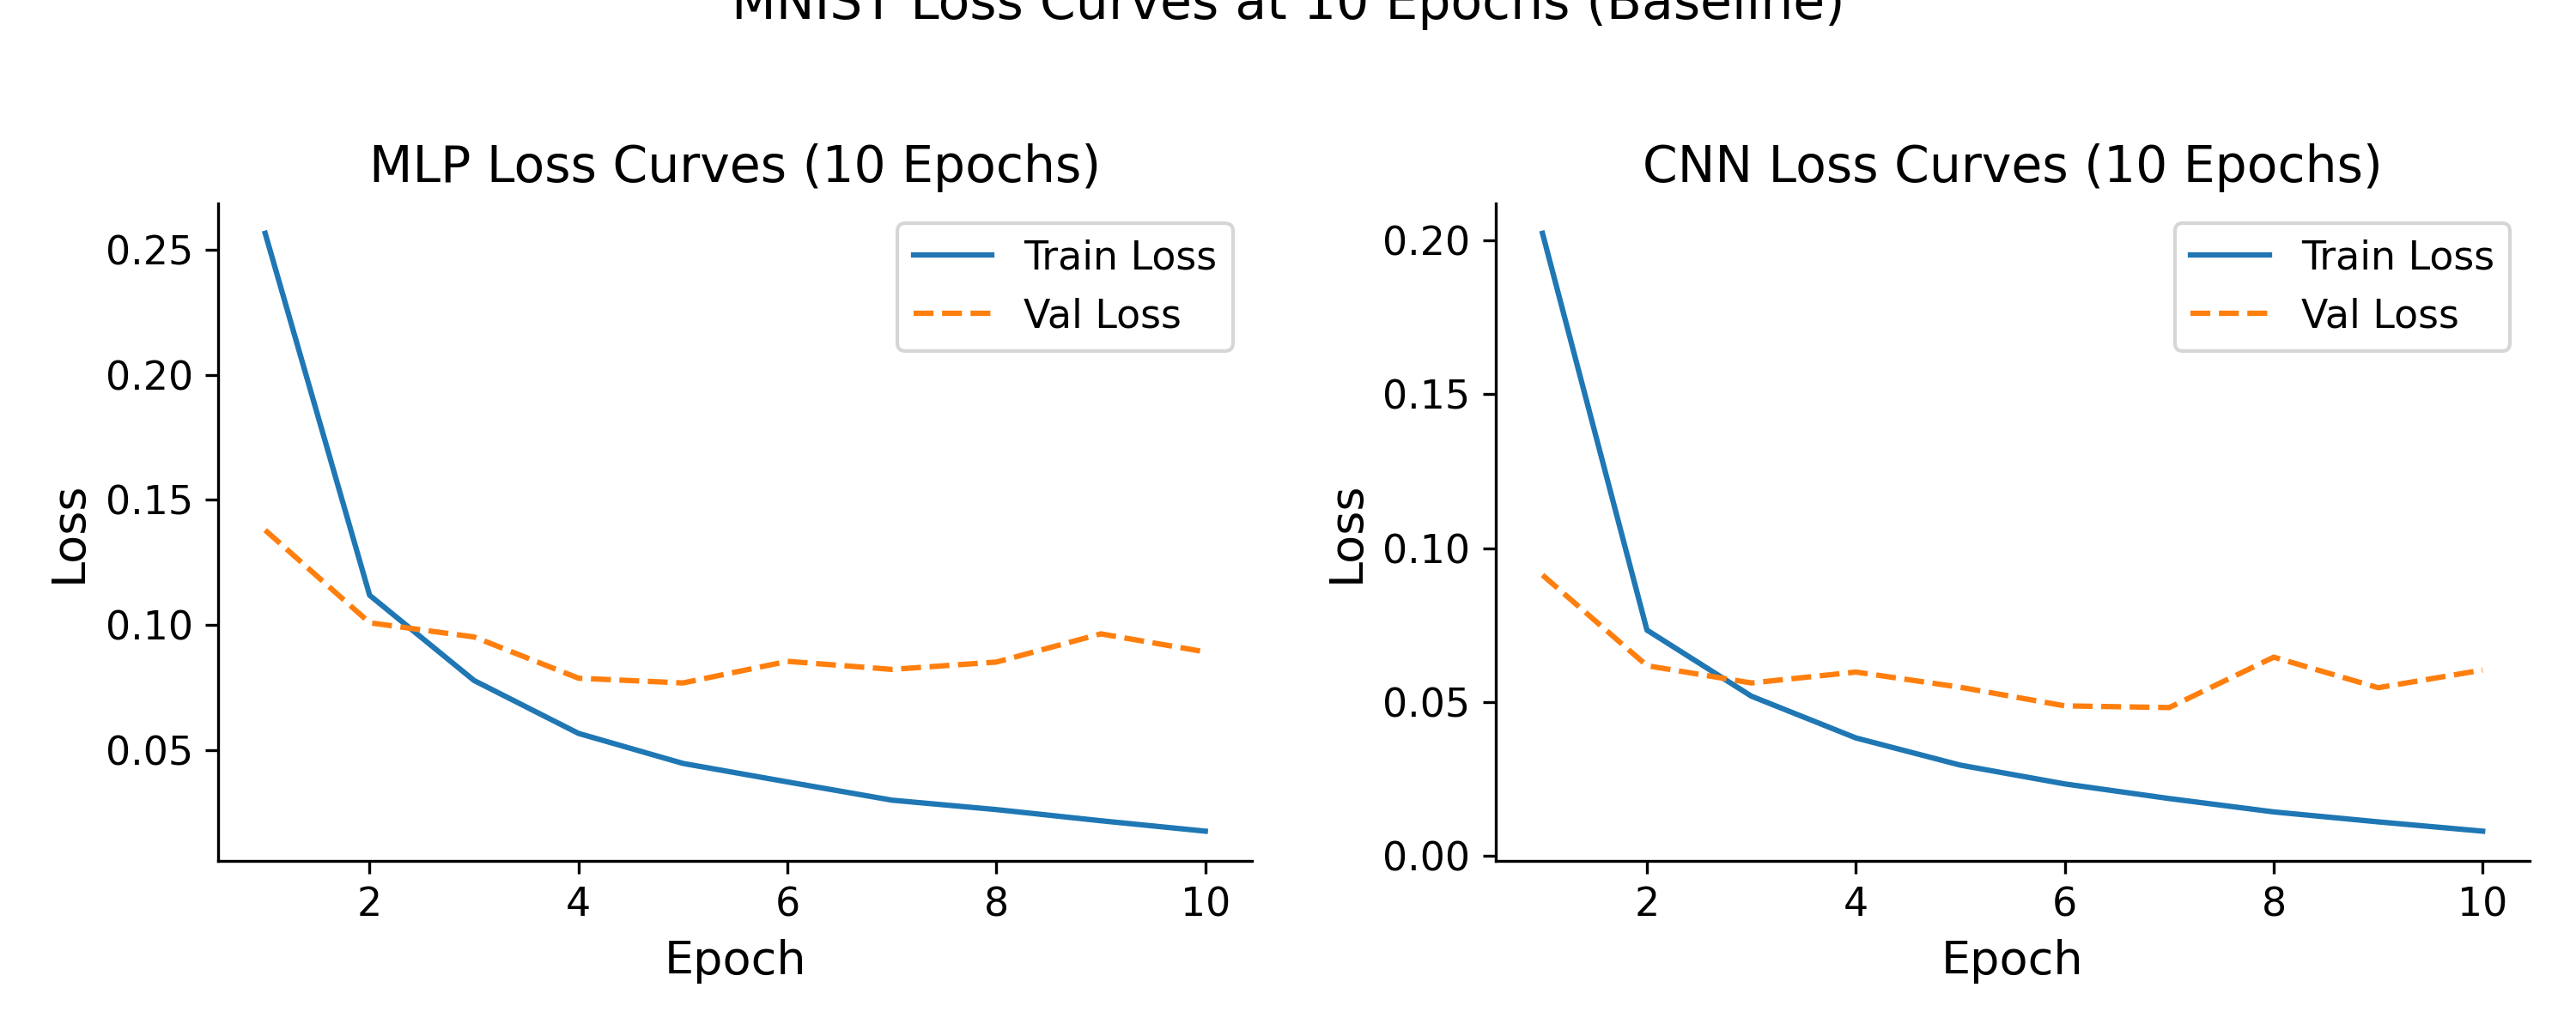
\includegraphics[width=0.48\textwidth]{mnist_loss_mlp_cnn_10_epochs.png}
  }
  \quad
  \subfigure[CGR vs.\ epoch for different budgets]{
    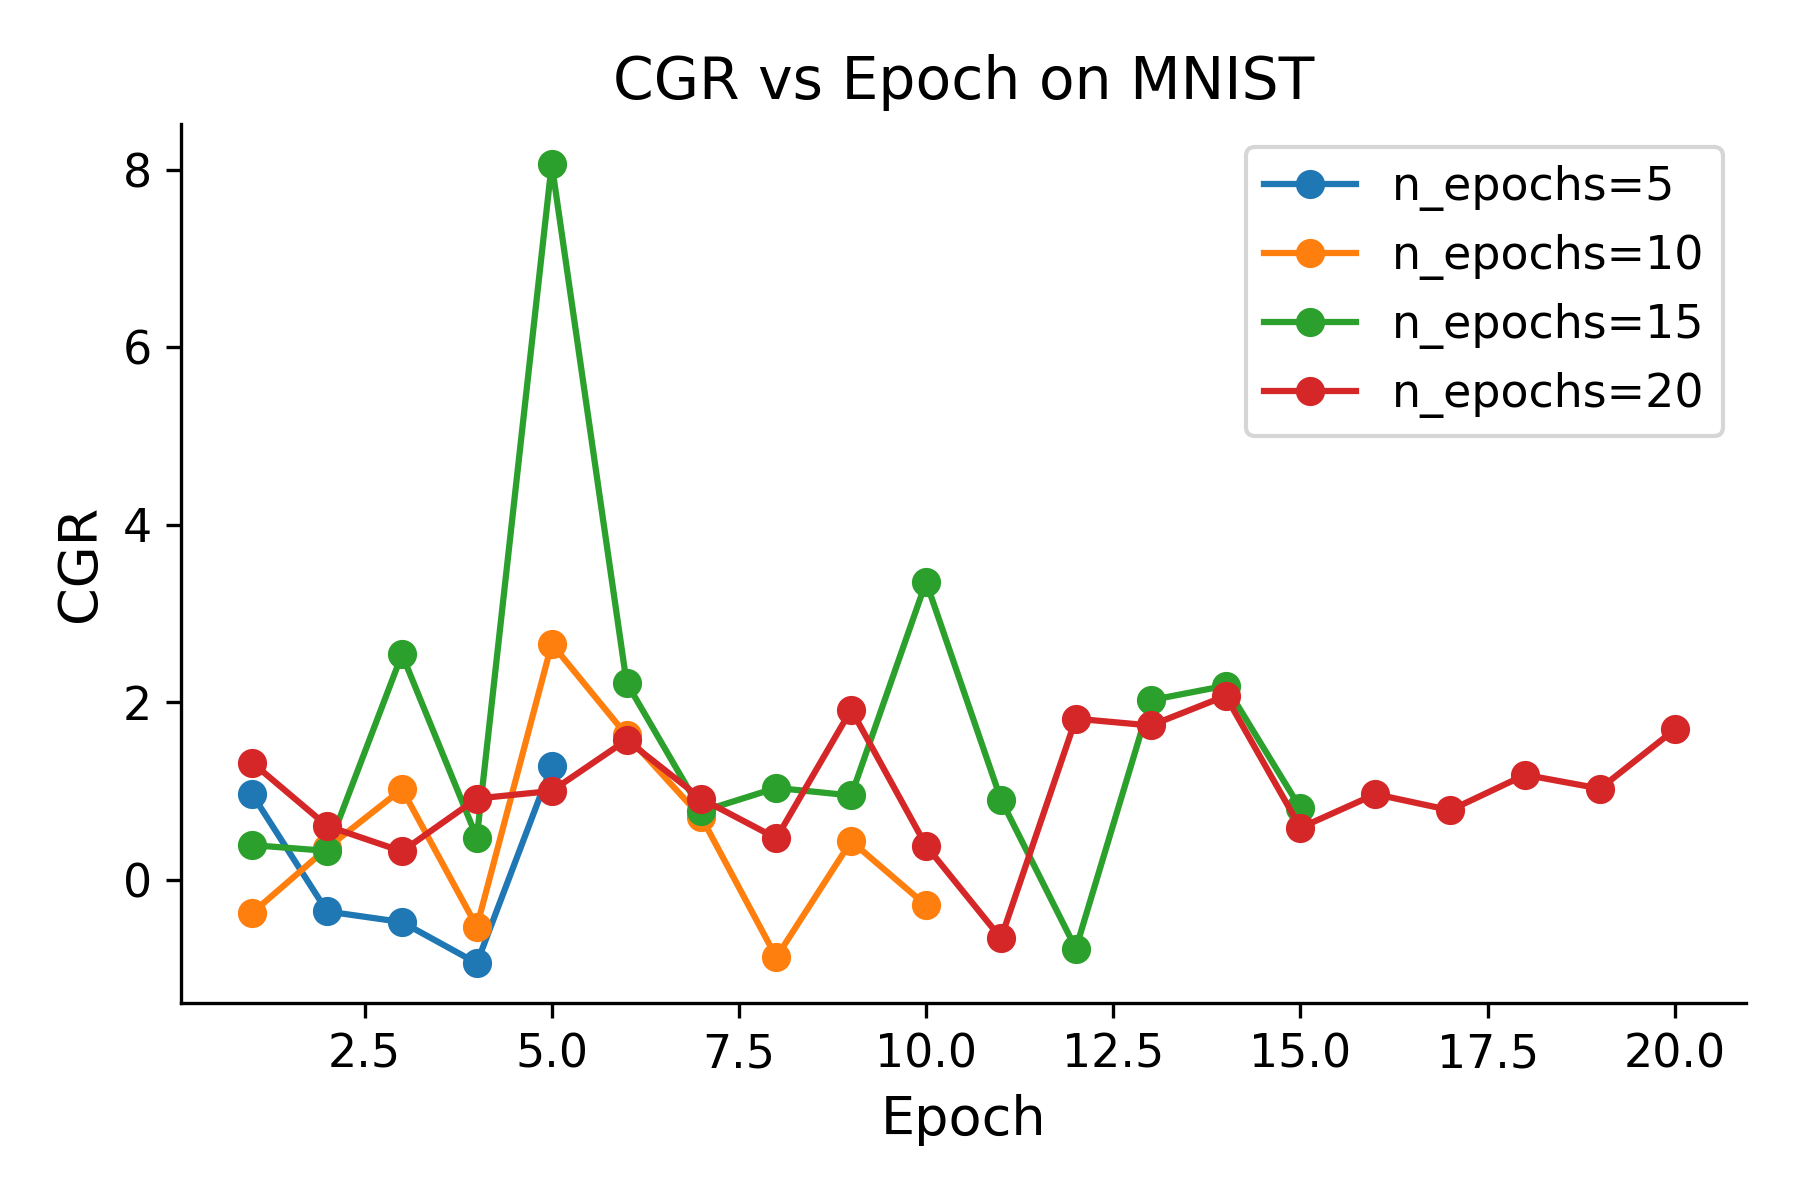
\includegraphics[width=0.48\textwidth]{mnist_cgr_vs_epoch.png}
  }
  \caption{MNIST rotation study. (a) Training (solid) and validation (dashed) loss for the MLP (left) and CNN (right). Overfitting occurs at epoch~5 for the MLP and epoch~3 for the CNN. (b) Challenge Gap Ratio exhibits budget-specific peaks around epochs 5–8, then flattens or declines as budgets increase.}
  \label{fig:mnist_loss_cgr}
\end{figure}

\subsection{Text Benchmark Discrimination}
\Cref{fig:text_accuracy}(a) presents final validation accuracies: RoBERTa leads by 1–2\% over BERT and DistilBERT on all tasks. In \cref{fig:text_accuracy}(b), we plot the Discrimination Score at the final epoch: SST2 yields the highest score ($\approx0.022$), followed by Yelp and AG News. These results confirm uneven aging across NLP tasks.

\begin{figure}[t]
  \centering
  \subfigure[Final validation accuracies]{
    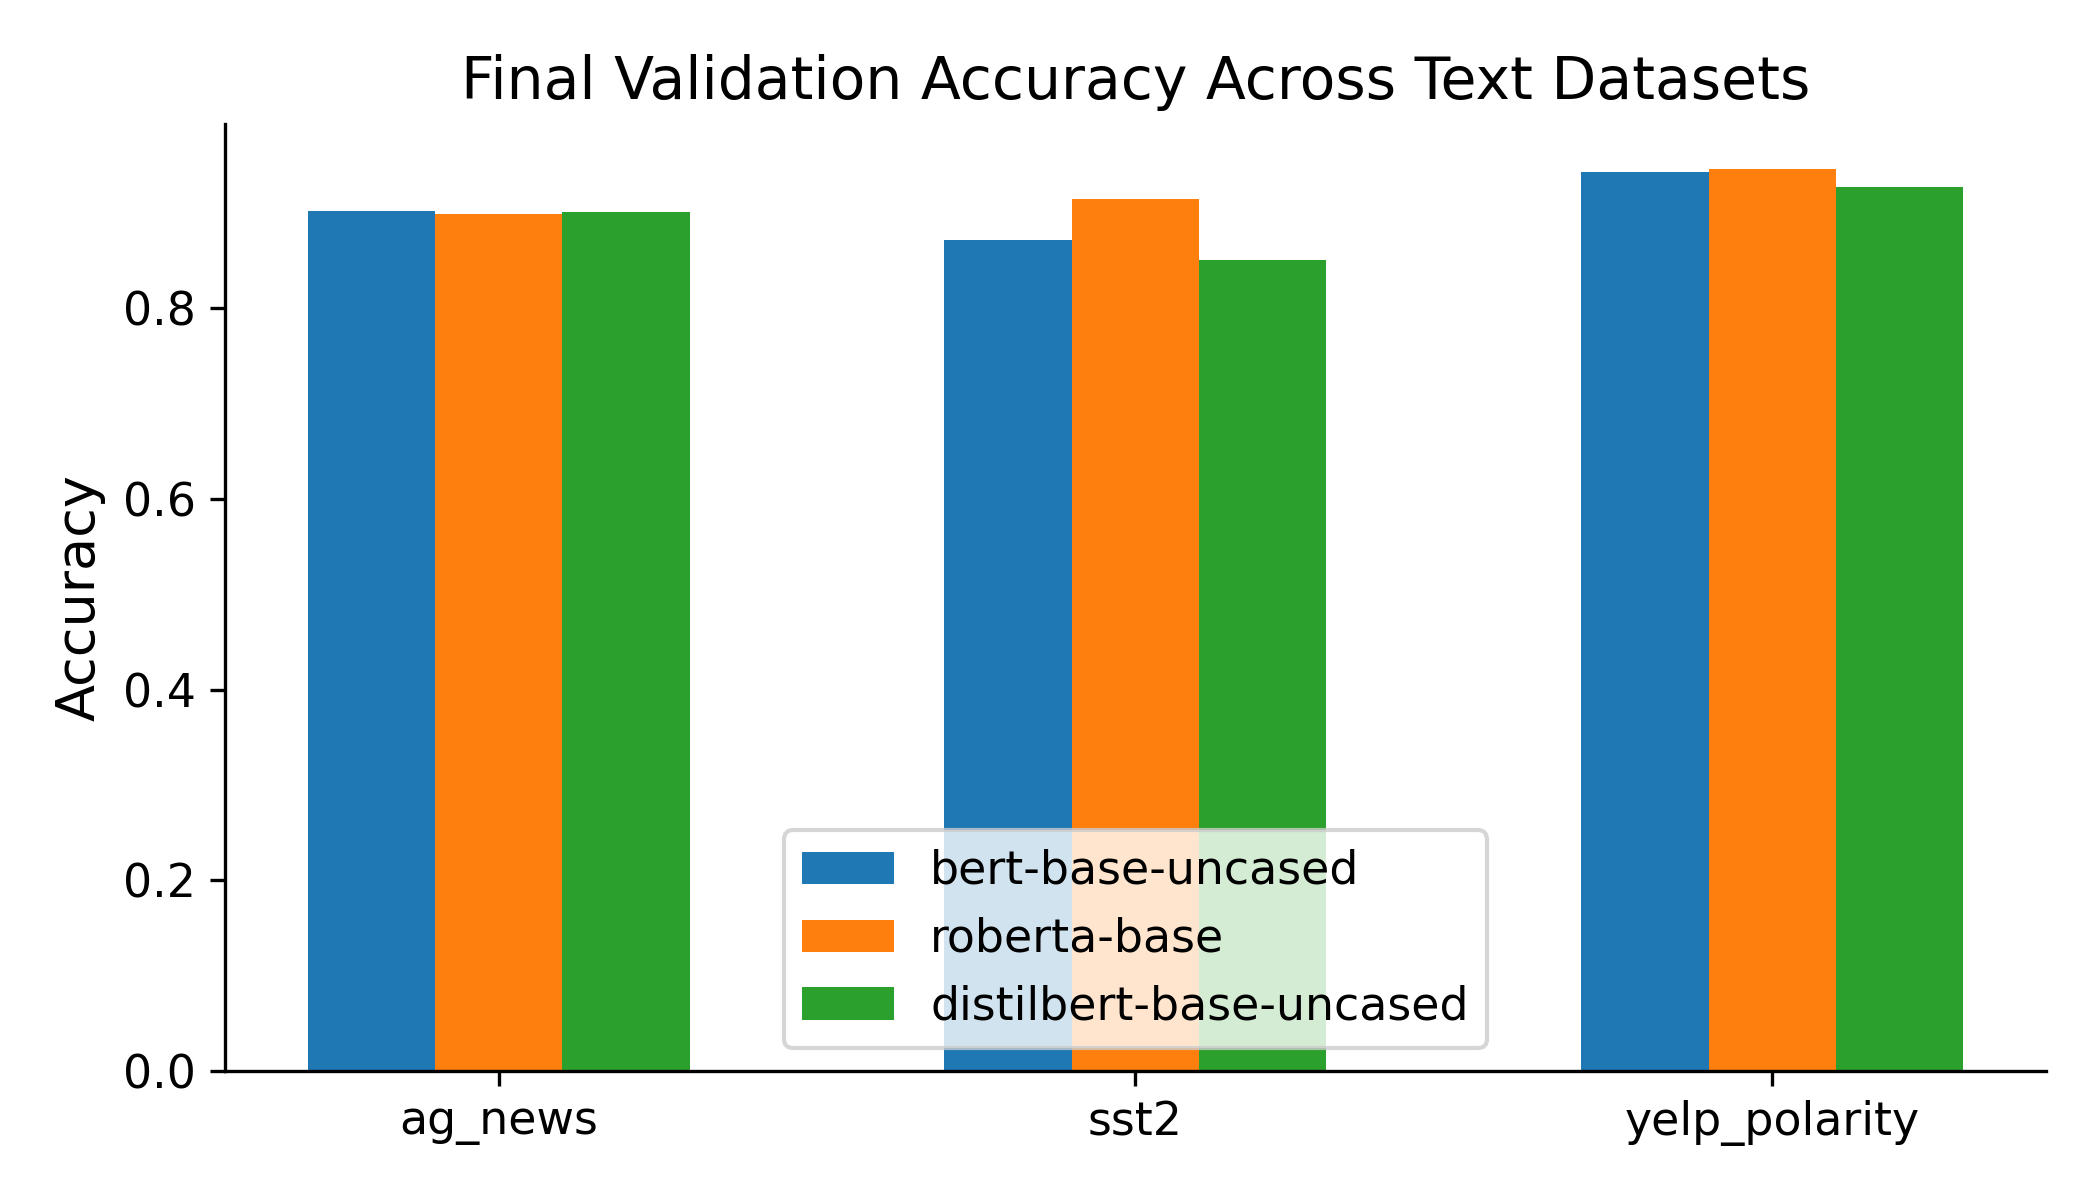
\includegraphics[width=0.48\textwidth]{final_val_accuracy_text.png}
  }
  \quad
  \subfigure[Discrimination Score at final epoch]{
    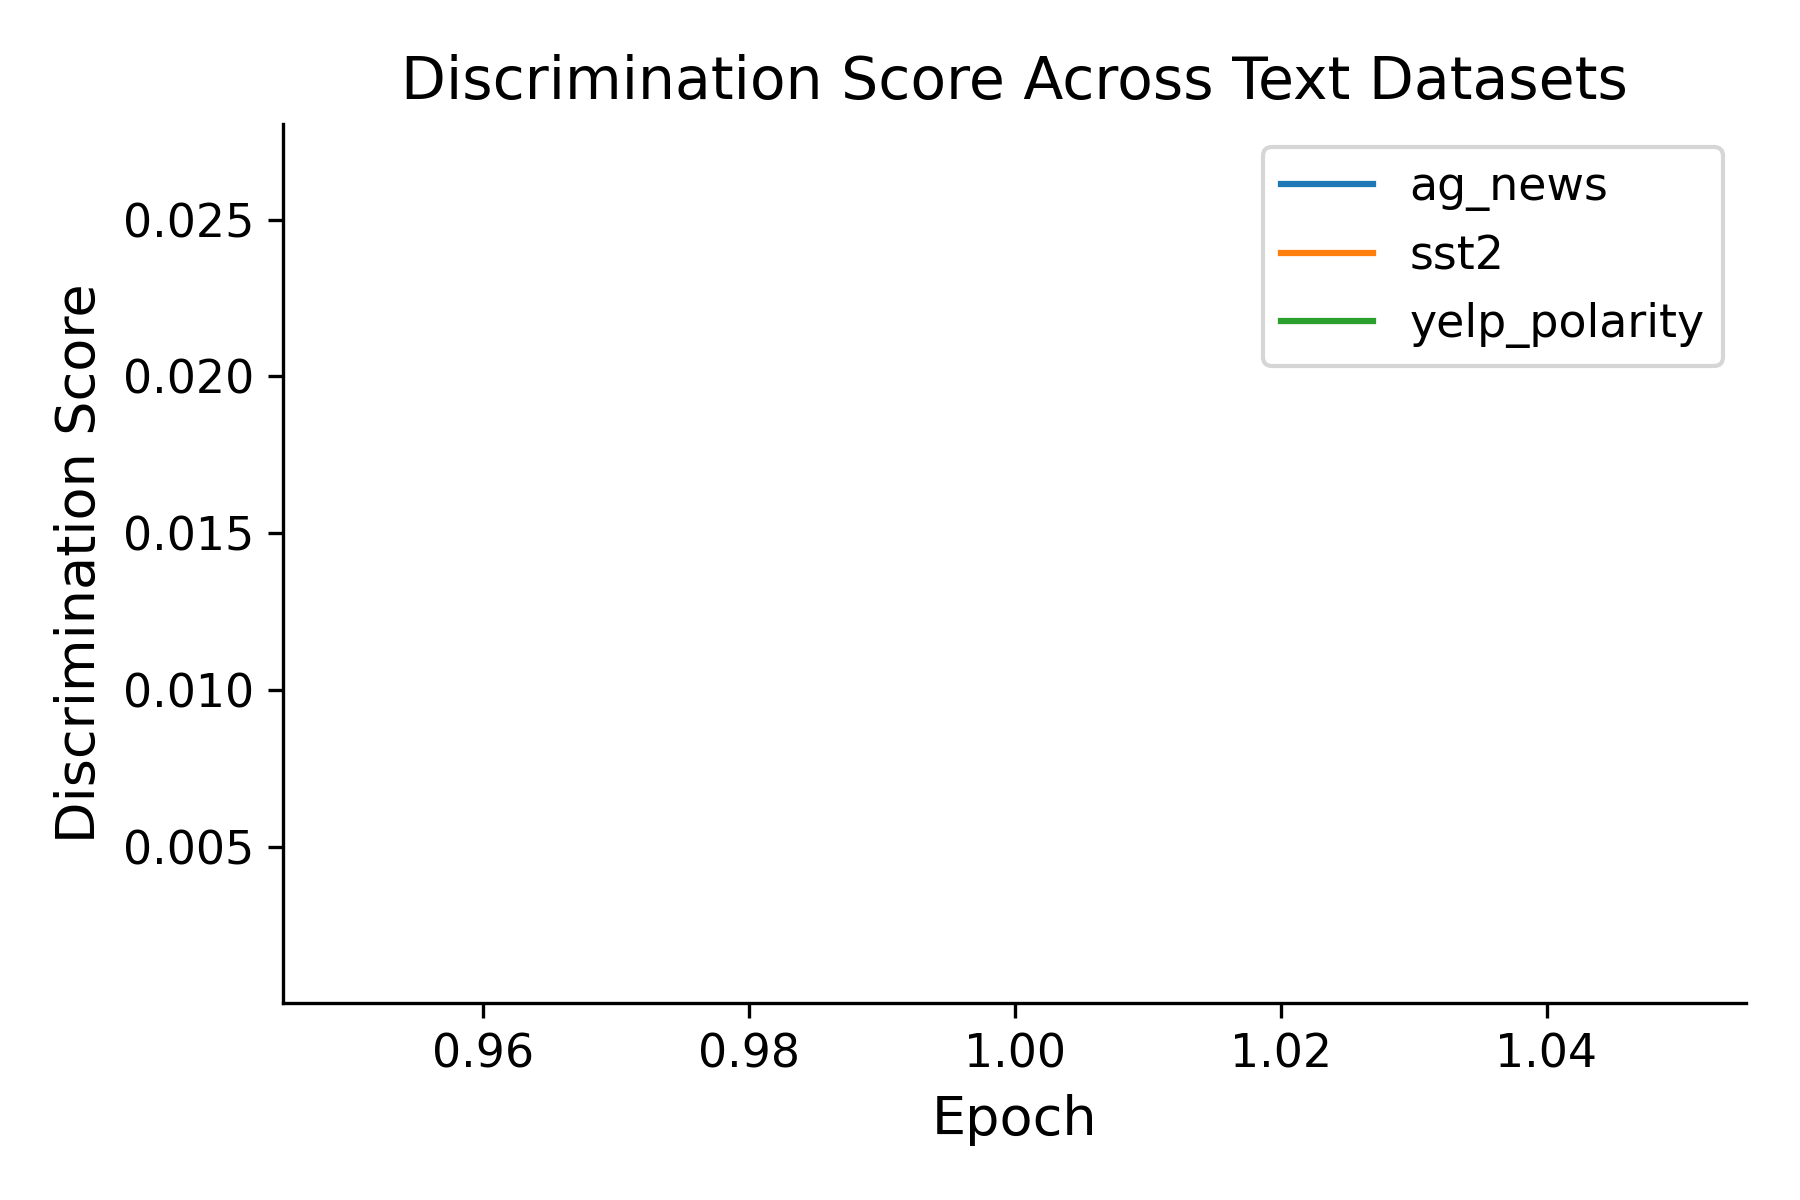
\includegraphics[width=0.48\textwidth]{discrimination_score_text.png}
  }
  \caption{Text classification study. (a) Accuracy of BERT, RoBERTa, and DistilBERT on AG News, SST2, and Yelp. (b) Discrimination Score (std.\ dev.\ of accuracies) at epoch~5: SST2 remains most discriminative.}
  \label{fig:text_accuracy}
\end{figure}

\subsection{Preliminary Synthetic Rejuvenation}
Applying our pipeline to MNIST rotation and AG News with FID<50 and perplexity<40 yielded candidate sets of 200–300 samples. However, rank-order correlations between original and rejuvenated leaderboards remained high (Kendall's $\tau>0.9$), and human evaluators flagged $\sim$30\% of synthetic texts as unnatural. These inconclusive results underscore challenges in balancing model uncertainty and real-world realism without manual curation.

\section{Conclusion}
We introduce a unified framework for measuring benchmark decay and an automated synthetic rejuvenation pipeline. Our analyses show that static vision and NLP benchmarks lose discriminative power in distinct ways: mid-training epochs optimize vision discrimination, while NLP tasks saturate unevenly. Early synthetic refresh helps marginally but falls short of manual quality. Future work will integrate human-in-the-loop validation and domain-aware generative strategies for sustainable, dynamic benchmarks.

\bibliography{references}
\bibliographystyle{iclr2025}

\appendix
\section*{Supplementary Material}
Additional ablations are shown in Figures~\ref{fig:hyperparameter_ablation} (learning rate scheduler and weight decay), \ref{fig:adv_mixup_ablation} (adversarial training and mixup), \ref{fig:aug_pool_ablation} (augmentation schemes and pooling), and \ref{fig:activation_ablation} (activation functions).

\begin{figure}[h!]
  \centering
  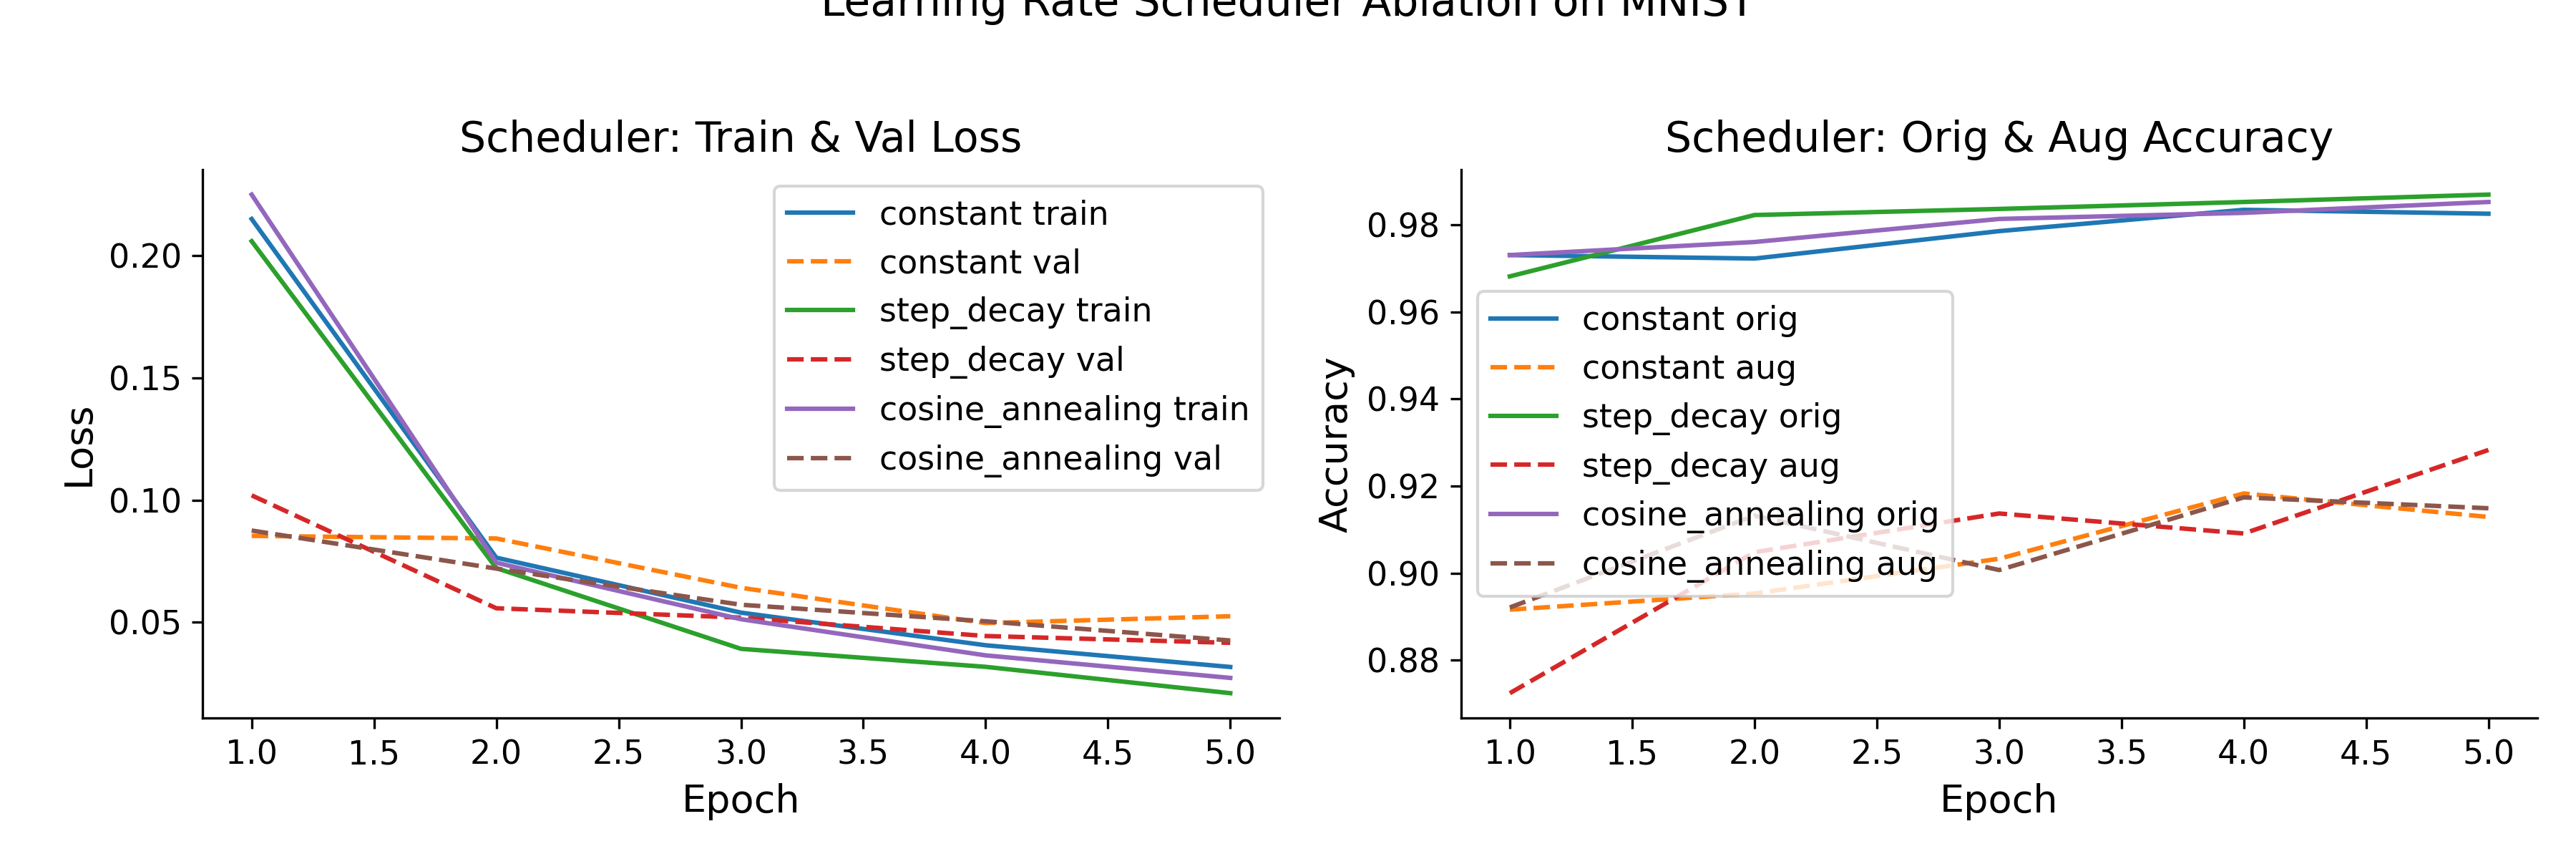
\includegraphics[width=0.48\textwidth]{lr_scheduler_ablation.png}
  \quad
  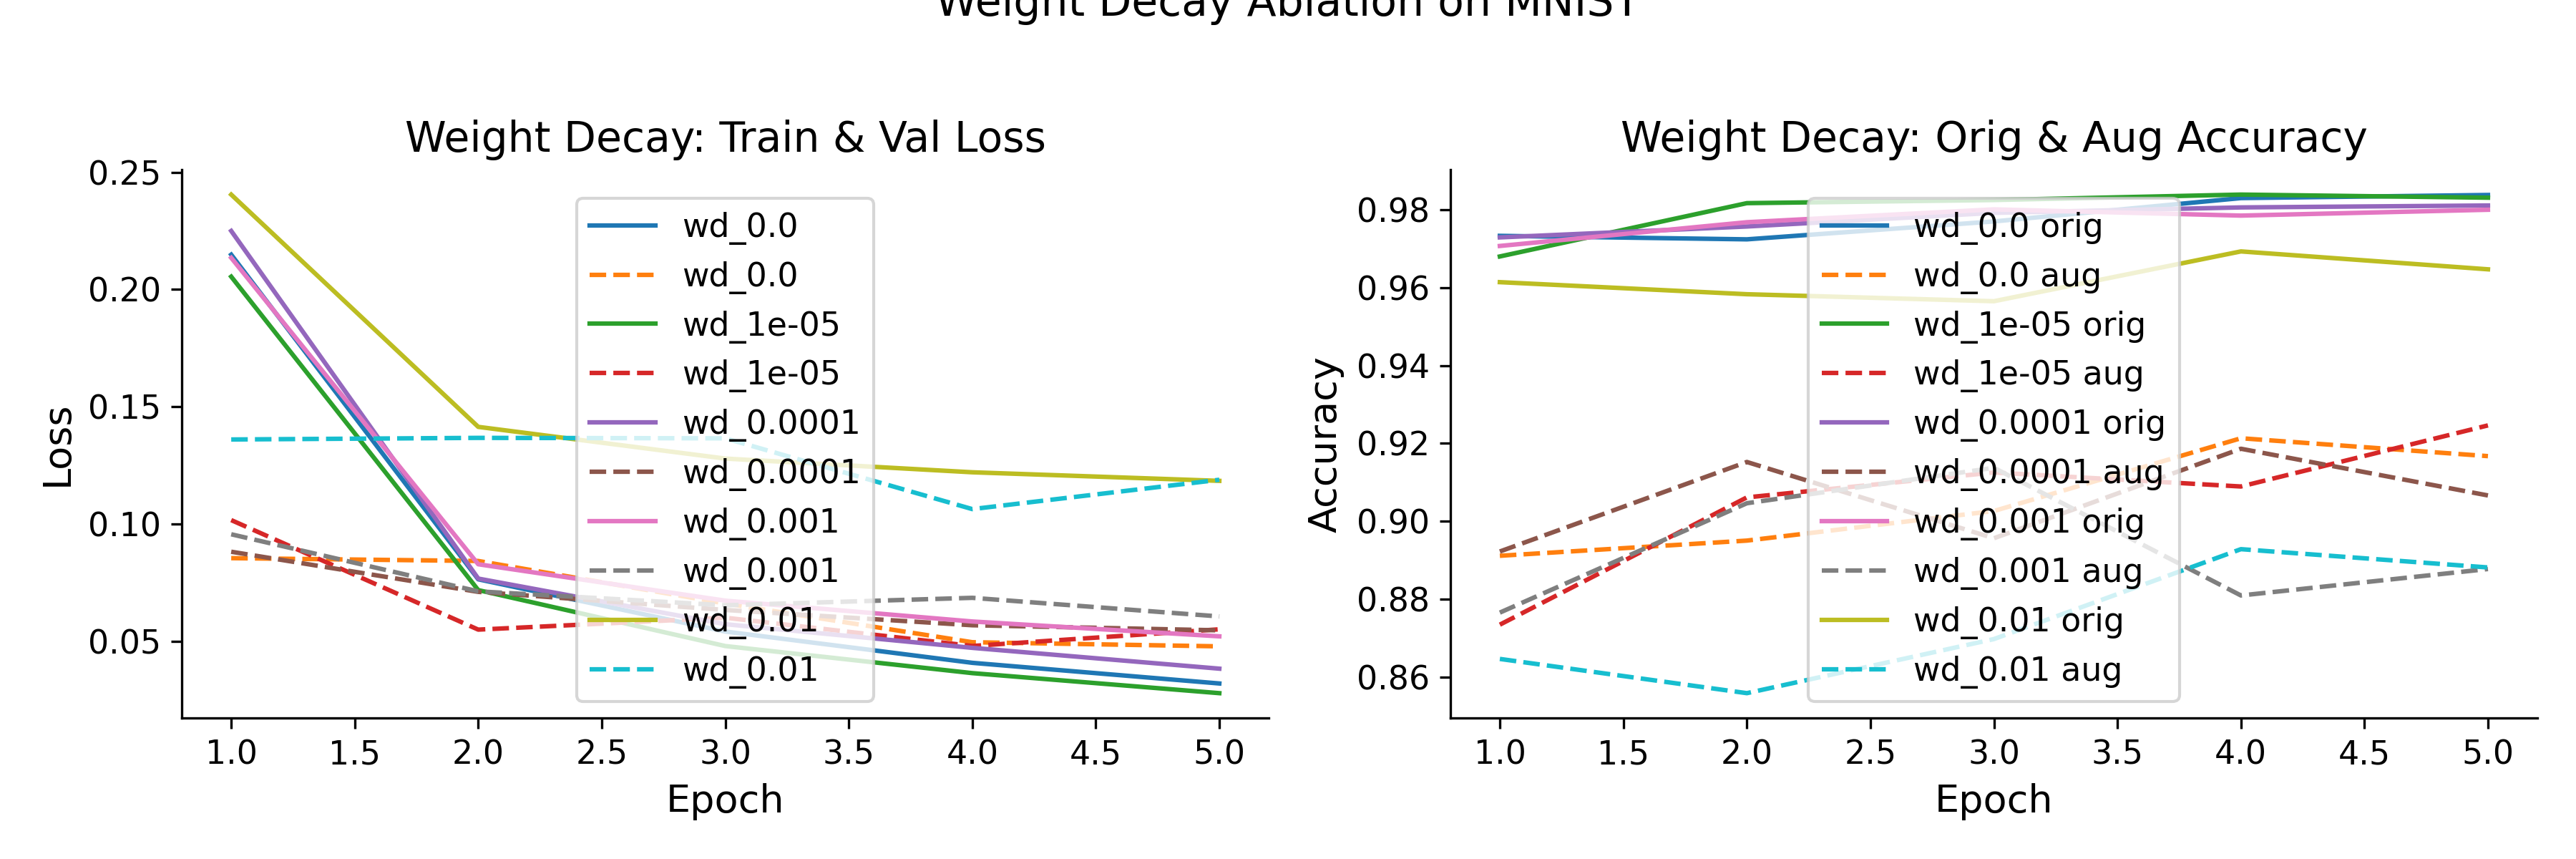
\includegraphics[width=0.48\textwidth]{weight_decay_ablation.png}
  \caption{Hyperparameter ablation: left shows scheduler variants (constant, step, cosine), right shows weight decay settings (0.0–0.1).}
  \label{fig:hyperparameter_ablation}
\end{figure}

\begin{figure}[h!]
  \centering
  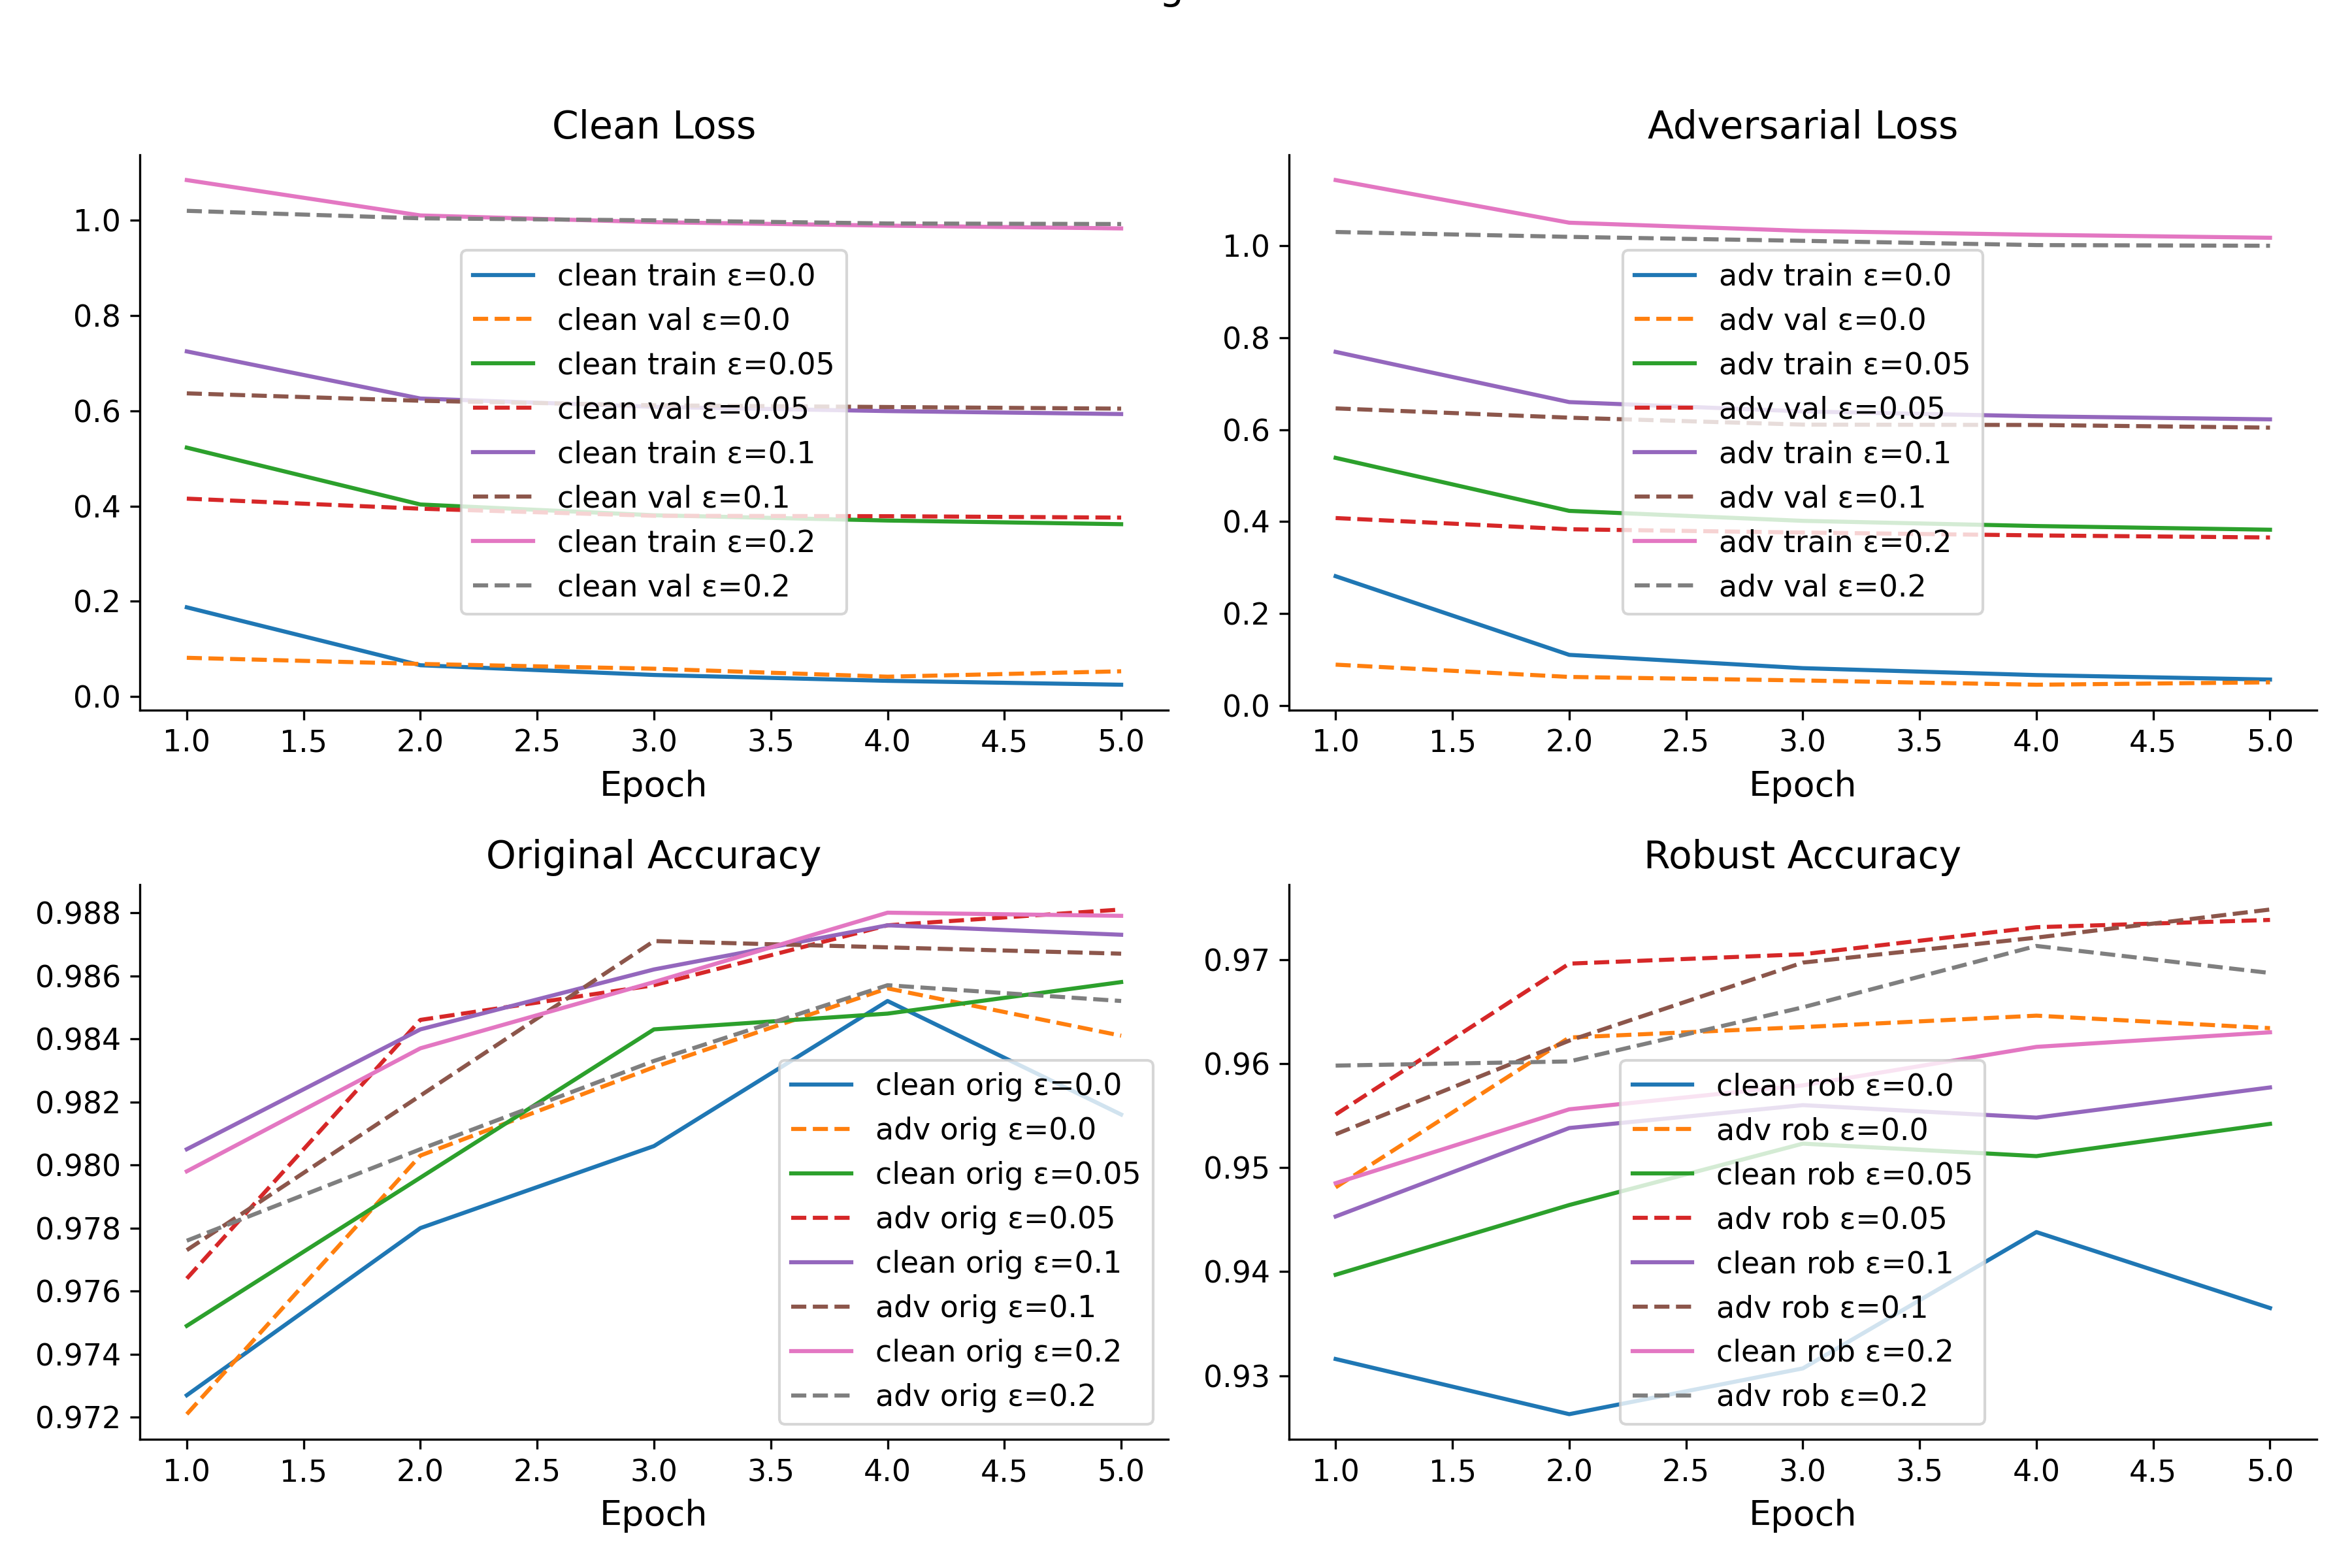
\includegraphics[width=0.48\textwidth]{adversarial_ablation.png}
  \quad
  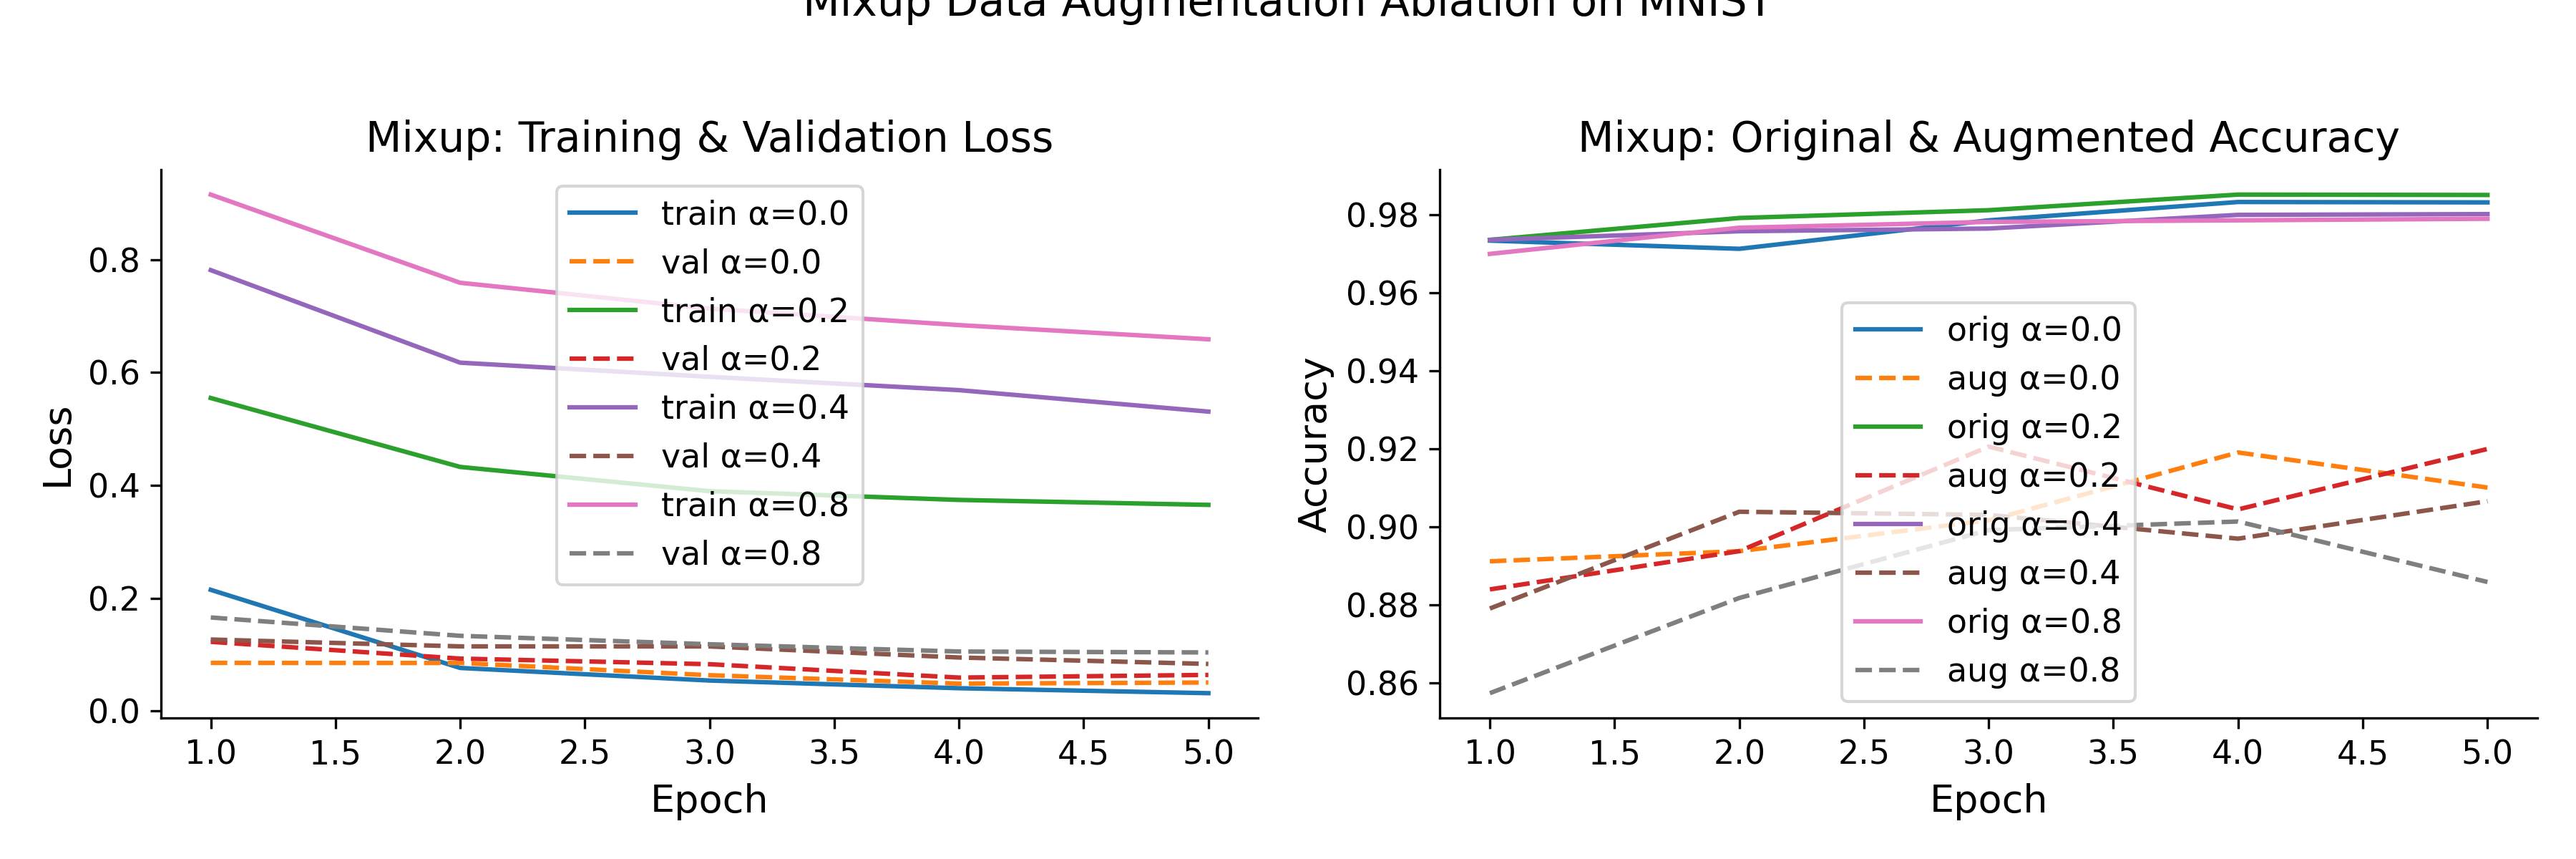
\includegraphics[width=0.48\textwidth]{mixup_ablation.png}
  \caption{Adversarial ($\epsilon$-perturbations) and mixup ($\alpha$) training ablations on MNIST rotation.}
  \label{fig:adv_mixup_ablation}
\end{figure}

\begin{figure}[h!]
  \centering
  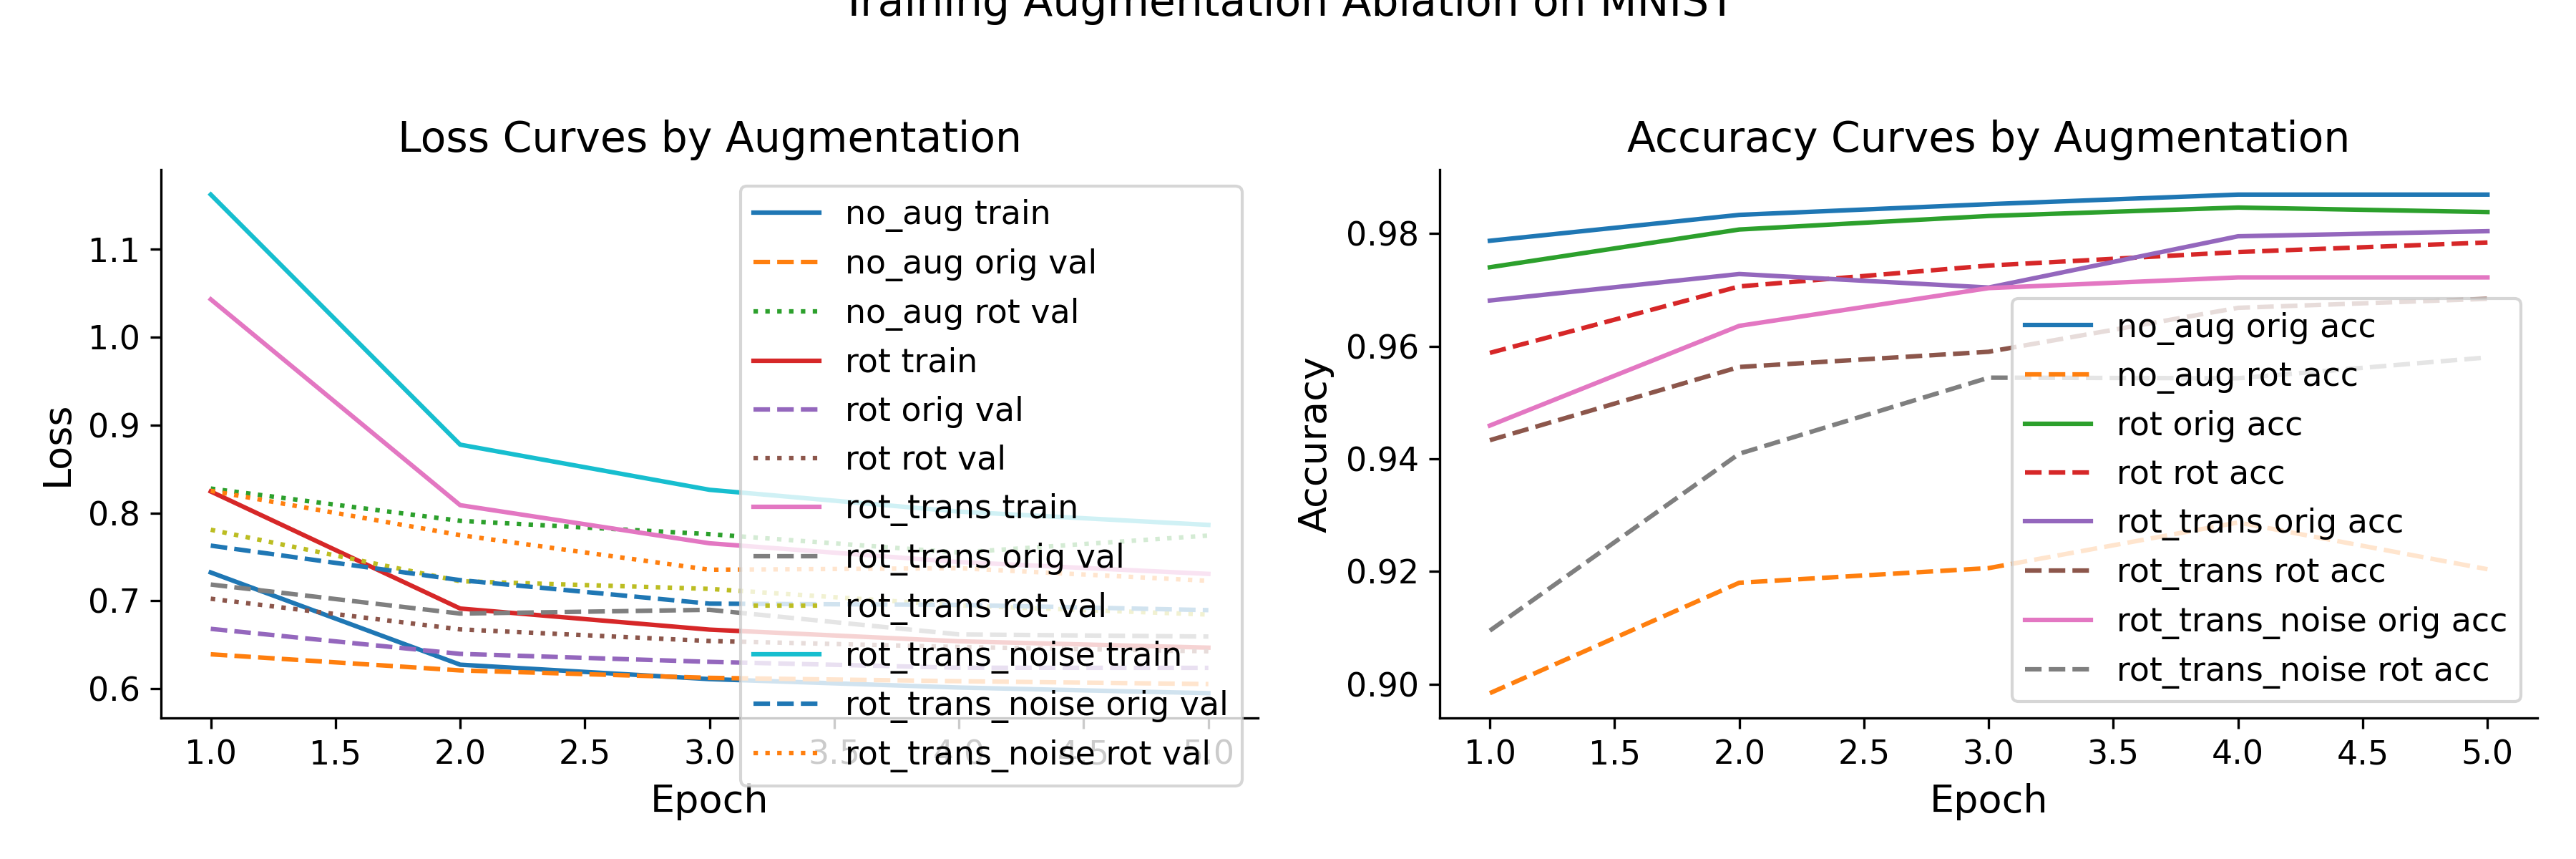
\includegraphics[width=0.48\textwidth]{augmentation_ablation.png}
  \quad
  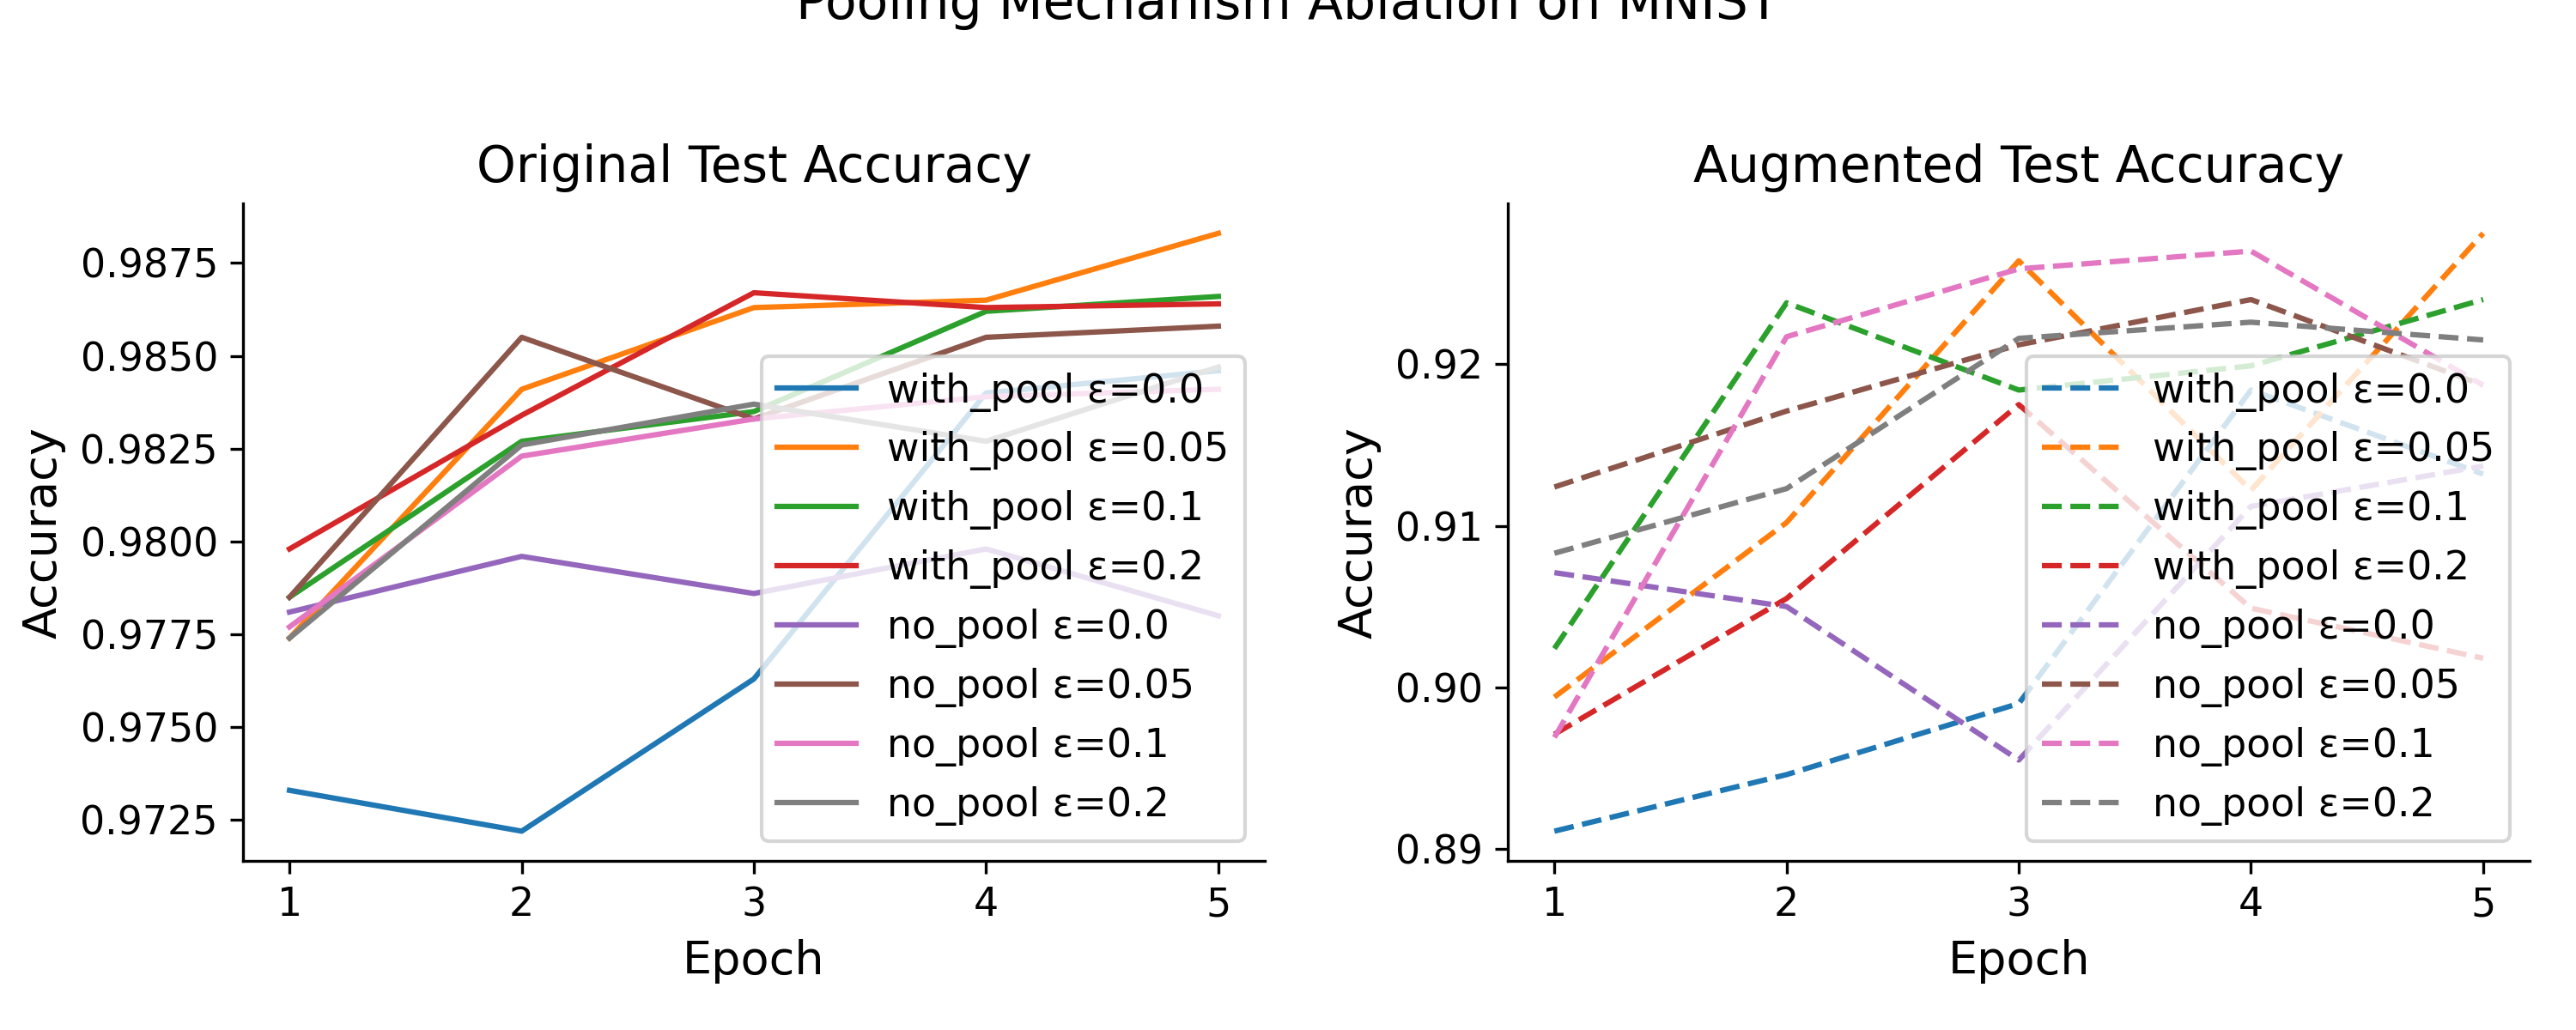
\includegraphics[width=0.48\textwidth]{pooling_ablation.png}
  \caption{General augmentation schemes (left) and pooling mechanism ($\alpha$-blending) ablations (right).}
  \label{fig:aug_pool_ablation}
\end{figure}

\begin{figure}[h!]
  \centering
  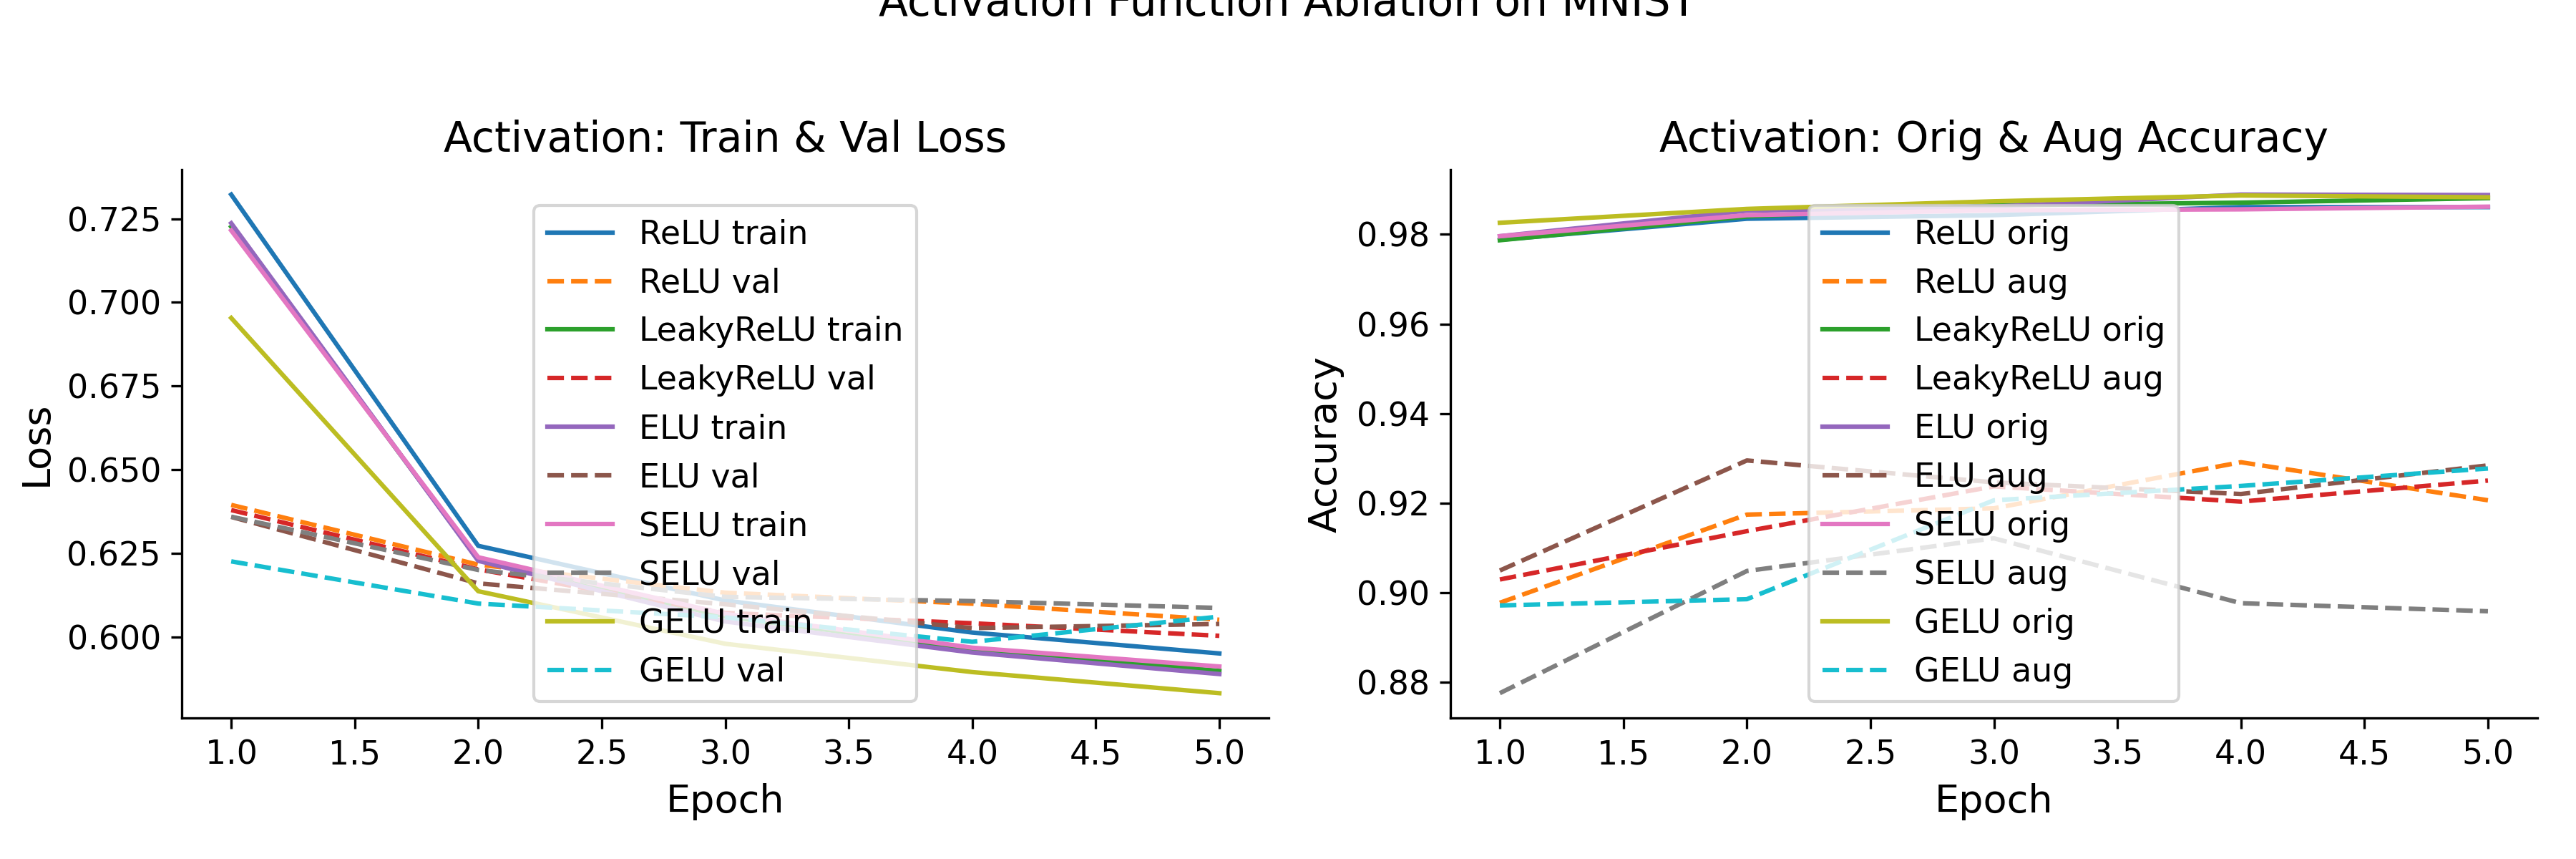
\includegraphics[width=0.6\textwidth]{activation_ablation.png}
  \caption{Activation function ablation on MNIST: training (solid) vs.\ validation (dashed) loss and original vs.\ augmented accuracy.}
  \label{fig:activation_ablation}
\end{figure}

\end{document}